\documentclass[12pt, a4paper]{report}
%\nonstopmode
\usepackage[english]{babel}
\usepackage[utf8]{inputenc}
\usepackage[T1]{fontenc}
\usepackage[british]{isodate}

\usepackage[usenames]{color}

\usepackage{graphicx}

% TOC
\setcounter{tocdepth}{3}
%\setcounter{secnumdepth}{4}

% Margins
\usepackage[hmargin={55pt, 55pt}, vmargin={2.8cm, 2.8cm}]{geometry}

%%% MATH
\usepackage{amsmath}
\usepackage{amssymb}
\usepackage{amsbsy}
\usepackage{amsthm}                % better theorem environments

% Captions
\usepackage[margin=1cm, labelfont=bf]{caption}
\usepackage{subcaption}
\usepackage{hyperref}

\usepackage[inline]{enumitem}

% Citations
\usepackage[round]{natbib}

% TikZ
\usepackage{tikz}
\usetikzlibrary{arrows,fit, positioning, shapes,
  calc, fadings, decorations.pathmorphing, hobby}

\tikzset{font=\tiny}
\tikzset{terminal/.style={circle, draw=black, fill=black, text=white}}
\tikzset{steiner/.style={circle, draw=black, fill=white}}
\tikzset{selected/.style={draw=red, ultra thick}}
\tikzset{root/.style={draw=cyan, ultra thick}}
\tikzset{subgraph/.style={font=\large, text=gray}}
\tikzset{snake it/.style={-stealth,
    decoration={snake, 
      amplitude = .2mm,
    segment length = 2mm,
    post length=0.9mm},decorate}}
\tikzset{snake node/.style={above=1mm,
    midway,
    text width=3cm,
    sloped,
    align=center}}
% Caption types

\DeclareCaptionType{formulation}[Formulation][List of formulations]

% TODO
\usepackage{todonotes}
\presetkeys{todonotes}{size=\tiny}{}
%%% Local Variables:
%%% TeX-master: "report"
%%% reftex-default-bibliography: ("lit.bib")
%%% End:


%\usepackage[titelside, en, nat]{ku-forside}
\usepackage[english, science, titlepage]{ku-frontpage}
%\usepackage{algorithm}
% \usepackage{algcompatible}
% \usepackage{bm}
% \usepackage{bbm}
% \usepackage{algpseudocode}
% \usepackage{arydshln}
% \usepackage[utf8]{inputenc} % æøå
% \usepackage[T1]{fontenc} % mere æøå
% \usepackage{verbatim} % så man kan skrive ren tekst


% \usepackage{graphicx}              % to include figures
% \usepackage{amsfonts}              % for blackboard bold, etc

% \usepackage{bm}
% \usepackage{pgf}
% \usepackage{fancyhdr}
% \usepackage{hyperref}
% \usepackage{stmaryrd}
% \usepackage{mathtools}
% \usepackage{multirow}
% \usepackage{listings}


% various theorems, numbered by section

\newtheorem{thm}{Theorem}[section]
\newtheorem{lem}[thm]{Lemma}
\newtheorem{prop}[thm]{Proposition}
\newtheorem{cor}[thm]{Corollary}
\newtheorem{conj}[thm]{Conjecture}

\newcommand{\nn}{\mathcal{N}}
\newcommand{\uu}{\mathcal{U}}
\newcommand{\bb}{\mathcal{B}}
\newcommand{\ee}{\mathrm{e}}
\newcommand{\rd}[1]{\mathrm{#1}}
\newcommand{\bd}[1]{\mathbf{#1}}  % for bolding symbols
\newcommand{\RR}{\mathbb{R}}      % for Real numbers
\newcommand{\ZZ}{\mathbb{Z}}      % for Integers
\newcommand{\BB}{\mathbb{B}}      % for Booleans
\newcommand{\PP}{\mathbb{P}}      % for Prob
\newcommand{\EE}{\mathbb{E}}      % for Expectation
\newcommand{\II}{\mathbbm{1}}      % for Indicator fun
\newcommand{\NN}{\mathbb{N}}      % for Prob
\newcommand{\col}[1]{\left[\begin{matrix} #1 \end{matrix} \right]}
\newcommand{\comb}[2]{\binom{#1^2 + #2^2}{#1+#2}}

\newcommand{\sint}[1]{\shortintertext{#1}}

\title{Prize-Collecting Steiner Trees}
\author{William Sprent -- \texttt{bsprent@gmail.com}}
\assignment{Master's Thesis} % Findes kun under 'titelside'
\subtitle{From the Perspective of the Prize-Collecting Travelling Salesman Problem}
\date{\today}
\advisor{Supervisors: Pawel Winter}

\begin{document}
\maketitle
~
\begin{abstract}
  The \gls{pcstp} in graphs is an NP-hard optimisation problem which involves
finding a connected subgraph which minimises the total sum of edge costs of
the subgraph and sum of vertex prizes for vertices not spanned by the subgraph.
It is a very well researched problem --- not least due to it being one of the
subjects of the \textit{11th DIMACS Implementation Challenge}.

In this master's thesis, we present a comprehensive survey of the research landscape
on the \gls{pcstp}. This involves a thorough look at some of the most interesting
and important algorithms for the \gls{pcstp}. Among the surveyed subjects are
powerful preprocessing routines, the widely cited Goemans-Williamson approximation
algorithm, and two state-of-the-art solvers.

We make use of this survey to consider the relation of the \gls{pcstp} other close
 problems, and take a new look at the younger and much less researched problem, the
\gls{mtp}. This problem is a generalisation of the \gls{pcstp} where instead of paying
static vertex prizes for unspanned vertices, a cost is now paid to \textit{assign}
unspanned vertices to the result subgraph.

For the \gls{mtp} we present a new \acrlong{ilp} formulation as well as a solver which
is able to generate exact solutions to the problem. Furthermore, we present a new
dataset based on previously released datasets for the \gls{pcstp}.

%%% Local Variables:
%%% TeX-master: "report"
%%% reftex-default-bibliography: ("lit.bib")
%%% End:

\end{abstract}

\tableofcontents
\clearpage

\chapter{Introduction}
\section{Background and Motivation}\label{sec:intro:background}
The hardest problems to solve do not necessarily have the most aethstetically pleasing solutions.
This is particularly true within the realm of NP-hard combinatorial optimisation problems.
Commonly, these are reformulated as \gls{ilp} problems, and solved through
branch-and-bound
by applying general purpose
\gls{mip} solvers. These solvers are then typically
fed with a bouquet of user callbacks for supplying
stronger lower bounds and good incumbents.

This is much akin to working with small disjoint building blocks
within a fixed framework, and when the problem changes, the framework stays
the same. Sometimes even some of the building blocks stay the same.

Hence, for many of these kinds of problems, finding exact solutions
involve using the same frameworks again and again.
Thus there exists a whole class of problems which are, to some point,
solved in the same manner.

\paragraph{Collecting Prize}
There is a family of combinatorial optimisation problems which involve
finding a subgraph which minimises total edge cost while paying a penalty
for not including vertices.

These problems generally live under the moniker of \textit{Prize-Collecting}
and were first introduced by \citet*{balas1989prize}
with the introduction of the \textit{\gls{pctsp}}. This problem is a generalisation of
the famous \gls{tsp}, relaxing its Hamiltonian tour constraint by instead applying penalities
to missed vertices and setting a minimum on collected \textit{prize}.

Perhaps unsurprisingly, this concept of collecting prize spread to another famous optimisation
problem, that is the \gls{stp}. This was done by \citet{Bienstock1993} in conjuction with
defining an approximation algorithm for the \gls{pctsp}. This variant of the \gls{stp},
aptly named the \gls{pcstp}, gained traction --- particularly with the
\textit{11th DIMACS Implementation Challenge} having Steiner Trees as its subject
\citep{DIMACS}.

At the onset of writing this thesis, the stated goal was to
survey the research done
on the \gls{pcstp}, and attempt to fill out any holes found with methods defined for the older
\gls{pctsp}. This was considered with the assumption that the older problem had
been more covered.
However, it turned out that the \gls{pcstp} had been \textit{far} more covered
by research with multiple exact algorithms
\citep{ljubic2005solving, leitner2016dual, gamrath2017scip},
approximation algorithms \citep{Bienstock1993,goemans1995general,Johnson:2000:PCS:338219.338637},
and primal heuristics \citep{canuto2001local,fu2014knowledge,akhmedov2016divide}
having been already proposed while the \gls{pctsp} had received little such attention
\citep{archetti2014chapter}.

As a consequence, the \gls{pcstp} with its mature field of research then appears to be a strong
starting point. The obvious choice, then, is to flip the equation and apply what we learn
from the \gls{pcstp} to the \gls{pctsp}.
However, there is another interesting problem to explore: \textit{the \gls{mtp}}.
The \gls{mtp} is a generalisation of the \gls{pcstp}
which involves finding the subgraph which minimises total edge cost summed with an
\textit{assignment cost} for assigning each vertex in the input graph to a vertex in
the subgraph.

The \gls{mtp} has only recieved much attention for the special case where the input graph is
a tree, giving us plenty of space to work in. Based on the evaluation that the tour constraint
puts the \gls{pctsp} at a further distance from the \gls{pcstp}, we make the \gls{mtp}
the secondary target of this thesis.
\section{Aim and Scope}
As we touch upon two slightly disjoint subjects, this thesis is split
in two parts.
\paragraph{Part I}

In the first part, we perform a
survey of the \acrlong{pctsp} where we report, detail, and bring intution to the most interesting
and/or effective methods for solving the \gls{pcstp}.
Our goal is not for this to be a comprehensive retelling
of all research done on the \gls{pcstp}, but to give a comprehensive \textit{overview} of
the kind of methods which are used to solve the \gls{pcstp}.
For example, we will not fully detail \textit{all}
heuristics or approximation algorithms for the \gls{pcstp},
but select those that we find most interesting or important.

The reader should be left with a good understanding of
what constitutes a state-of-the-art method for solving the \gls{pcstp}.

\paragraph{Part II}

In the second part, we widen our lenses and look at problems which are related to the \gls{pcstp},
but still from the perspective of
the \gls{pcstp}.
First we will take a superficial look at the closest problem,
before taking a deep dive in the \acrlong{mtp} for which
we proprose an \gls{ilp} formulation, a new dataset, and a solver.

Our aim is to uncover how the \gls{pcstp} relates to other problems
both with regards to the nature of the problems themselves and state of
research.

Furthermore, we wish to examine how translatable results made for the \gls{pcstp} are for similar problems.
In other words, we ask the question,
``Can research on one combinatorial optimisation problem be applied directly, or at least
serve as a good starting point for solutions to another such problem?''

\medskip\noindent
Overall, we first take a look at a well-understood problem with a mature field of reasearch and collect
the main points of knowledge in one place. Then we turn our view to problems with younger research fields
and see how the former relates to the latter.

In the end, we aim to see how well state-of-the-art methods used to solve an NP-hard combinatorial
optimisation problem can be utilised to solver another NP-hard problem when the problems are particularly
similar in formulation.

\section{Related Work}
Besides the research we cover through our survey in
Part~\ref{part:survey} of this thesis,
there has been some recent work which is closely related
 to what we present. Particularly, there has been some in surveying the
\acrlong{pcstp} from different angles.

\citet*{rehfeldt2016reduction} present a comprehensive study of all preprocessing routines
for the \gls{pcstp} and the Node-Weighted Steiner Tree Problem. This is similar in scope to
Section~\ref{sec:solving:pre} in this thesis. The reader is encouraged to visit their paper
if they wish to see a more theoretical and comprehensive look at preprocessing routines for
the \gls{pcstp}. We aim to complement this with a slightly more intuitive description of the
routines.

\citet*{sun2018classical} presents a survey of the practical applications of the \gls{pcstp}.
In their thesis, they first perform a short summary of the historical perspective of
solving the \gls{pcstp}. Their main contributions include
a detailed look at the applications
of the problem in real world scenarios.

\section{Notation}\label{sec:intro:notation}

Throughout this thesis, we will make repeated use of some shorthand notation, particularly
with respect to graphs and decisions vectors.

\paragraph{Graphs}

We define the adjacency function $\delta : V \to \mathcal{P} (E)$ on undirected graphs as
the function which given the index of a vertex, returns all adjacent edges, that is
\[\delta(i) = \{(i,j) \mid j \in V \wedge (i, j) \in E\}\mathnormal{.}\]
On a directed graph, this is replaced by two functions
$\delta^+ : V \to \mathcal{P} (A)$
and $\delta^-: V \to \mathcal{P} (A)$.
The former returns all vertices, $j$, for which there exists an arc
which starts in the input vertex, $i$, and terminates in $j$, that is
\[\delta^+(i) = \{(i, j) \mid j \in V \wedge (i, j) \in A\}\mathnormal{.}\]
Correspondingly, $\delta^-$ then returns the set,
\[\delta^-(i) = \{(j, i) \mid j \in V \wedge (j, i) \in A\}\mathnormal{.}\]
When we are not interested in adjacent edges, but instead neighbouring vertices,
we may use $\delta(v)$ to mean the set of vertices which are neighbours to $v$.
This will be clear in usage.


When given some subset of vertices, $S \subseteq V$, as input,
$\delta(S)$ returns all edges which span the cut $(S, V \setminus S)$.
Thus we have $\delta : \mathcal{P}(V) \to \mathcal{P}(E)$, with
\[\delta(S) = \{(i,j) \in E \mid i \in S \wedge j \in V \setminus S\}\mathnormal{.}\]
And for directed graphs we have, $\delta^+ : \mathcal{P}(V) \to \mathcal{P}(A)$, with
\[\delta^+(S) = \{(i,j) \in A \mid i \in S \wedge j \in V \setminus S\}\mathnormal{,}\]
and $\delta^- : \mathcal{P}(V) \to \mathcal{P}(A)$, with
\[\delta^-(S) = \{(i,j) \in A \mid i \in V \setminus S \wedge j \in S\}\mathnormal{.}\]

\paragraph{Decision Vectors}

When working with \gls{ilp} models of graph problems, we often need to sum over variables
related to edges or vertices. For example, let $x_{ij}$ be $1$ if the edge $(i,j) \in E$
is part of a solution and $0$ if not, and let $L \subseteq E$ be some subset of edges.
Then the \textit{function} $x : \mathcal{P} (E) \to \NN$ returns the number of edges
 in $L$ which was selected in the solution defined by $x$,
 \[x(L) = \sum_{(i, j) \in L} x_{ij}\mathnormal{.}\]
 If $x_{ij}$ is a real number, then $x(L)$ returns a real number as well.

\clearpage
\glsaddall
\printglossaries

%%% Local Variables:
%%% TeX-master: "report"
%%% reftex-default-bibliography: ("lit.bib")
%%% End:

\chapter{Background}
\label{chap:BG}
\section{Combinatorial Optimisation}
\label{sec:CO}
\section{The Steiner Tree Problem}
\label{sec:STP}

\section{The Traveling Salesman Problem}
\label{sec:TSP}

bla bla


\part{Survey}

\chapter{Steiner Trees}
\label{chap:steiner-trees}

bla
\chapter{Solving the Prize-Collecting Steiner Tree Problem}
\label{chap:solving}

In this chapter, we will present a survey of methods used to solve the Prize-Collecting Steiner Tree Problem. Due to the nature of solving
NP-hard combinatorial optimisation problems, this involves the the mixing and matching of methods within larger frameworks.
 After a rundown of the history of solving the PCSTP in section \ref{sec:solving:history}, we will present the following:
\begin{itemize}
\item Section \ref{sec:solving:pre} presents preprocessing algorithms used to reduce instance sizes.
\item Section \ref{sec:solving:approx} presents approximations for solving the PCSTP.
\item Section \ref{sec:solving:heuristics} presents heuristics for solving the PCSTP.
\item Section \ref{sec:solving:lower} presents methods used for generating lower bounds.
\item Section \ref{sec:solving:exact} presents frameworks and combinations of the above used find exact solutions
   to the PCSTP.
\end{itemize}

\section{History}
\label{sec:solving:history}

Solutions to the PCSTP were first explored by \cite{Bienstock1993} who
proposed a 3-approximation algorithm based on Christophides algorithm for the TSP.
This was later improved to 2-approximation algorithm by
\cite{goemans1997primal} using a primal-dual method,
which was refined and implemented
for faster runtimes and typically better
bounds by \cite{Johnson:2000:PCS:338219.338637}.

\cite{canuto2001local} presented a primal heuristic based on multi-start
local search with pertubations and path relinking.

An ILP formulation based on the General Subtour Elimination Constraint (GSEC) formulation of the Travelling Salesman Problem was
stated by \cite{lucena2004strong}, who presented an algorithm for solving the LP relaxation of the GSEC formulation using
a separation procedure as a method for generating a strong lower bound for the PCSTP. Similarly, \cite{Ljubic:2004:memetic}
presented a memetic algorithm using tournament selection and mutation. They additionally presented an ILP formulation of the Steiner
 Aborescence Problem, based on cuts, the LP-relaxation of which was solved on a subgraph extracted from the memetic algorithm to
 improve the solutions as a postprocessing step.

 \cite{ljubic2005solving} proposed the first full framework for solving the PCSTP to optimality.
 This was done by solving
 equivalent SAP instances through branch-and-cut. Solving the LP-relaxation of a cut-formulation of the SAP with a
 a separation procedure was used to generate lower bounds.
  Furthermore, they presented a set of real-world problem instances for the PCSTP based on network layout in Berlin.

  \cite{lucena2004strong}, \cite{Ljubic:2004:memetic}, and \cite{ljubic2005solving} all applied preprocessing routines
  -- known as reduction tests -- to their input graphs to reduce the size of instances.
  These were originally gathered for
  the Steiner Tree Problem by \cite{duin1989edge,duin1989reduction},
  but no reduction tests had been stated and proven for the PCSTP
  until \citeauthor{uchoa2006reduction} did so in \citeyear{uchoa2006reduction}.
  \citeauthor{uchoa2006reduction} revisited
  reduction tests originally defined for the STP,
  but also introduced a new
  novel way of determining distances between nodes,
  allowing for stronger reduction tests.

  The 11th DIMACS challenge on Steiner tree problems\footnote{\url{http://dimacs11.zib.de/}}
  brought not only a new set of instances for the PCSTP, but
  also a new wave of contributions.

  Solving the PCSTP by transforming instances into equivalent problems in directed graphs
  was revisited by \cite{leitner2016dual} and \cite{gamrath2017scip}.
  \cite{leitner2016dual} transformed instances into the Asymmetric Prize-Collecting Steiner Tree Problem (APCSTP)
  and employed a
  branch-and-bound framework generating lower bounds with a dual ascent method which was originally presented by \cite{wong1984dual} for the SAP, and
  generating incumbents with
  a shortest-path primal heuristics.
  \cite{gamrath2017scip} presented SCIP Jack -- an exact solver for STP variants based on the solver (of the STP, by way of SAP) presented by
  \cite{koch1998solving} and the MIP solver, SCIP \footnote{\url{http://scip.zib.de/}}.
  Preprocessing routines were natively applied to PCSTP instances before transforming them into SAP instances.
  The SAP was formulated as an
  ILP in a so-called \textit{Flow-Balanced Directed Cut Formulation}. The general branch-and-bound
  procedures of the SCIP optimization suite were
  then employed together with a contraint separation procedure defined in \cite{koch1998solving}.

  Developments were also made in field of heuristics for the PCSTP. \cite{fu2014knowledge} presented a tabu search and a neighbourhood definition
  using a new \textit{vertex swap} operation.
  \cite{akhmedov2016divide} presented a clustering heuristics for dividing PCSTP into subproblems,
  and additionally a
  reimplementation of the solver by \cite{ljubic2005solving} which was used to solve problems defined by the subgraphs. Additionally, they presented
  applications for the PCSTP within biology.
  \cite{biazzo2012performance} explored the performance of the cavity method on the PCSTP.
  
 \section{Preprocessing}
 \label{sec:solving:pre}
Applying preprocessing routines to heavily reduce input graphs is a common technique which has been proven succesful in many cases both for instances of the \gls{stp}
\citep{koch1998solving}
and instances of the \gls{pcstp}
\citep{lucena2004strong,canuto2001local,ljubic2005solving, gamrath2017scip}. %TODO: MORE
These routines make use of proven invariants to remove and contract edges as well as choose edges before applying the any main procedure.
A set of common preprocessing routines are applied in different manners in literature, mainly differentiated by:
\begin{enumerate}[label=\alph*)]
\item which routines to apply,
\item in which order, and
\item when to recursively apply routines and how many times.
\end{enumerate}
Preprocessing routines can be very effective. For example, the preprocesing routine presented by \cite{koch1998solving} for the \gls{stp} removes
up to 98\% of edges in some instances. In this section, we will first give a full overview of existing preprocessing methods for the \gls{pcstp},
 including proofs of validity,
 and then summarize their usage in recent literature.

 In the following, we will denote any edge or vertex (or part of a graph) as \textit{redundant} if there exists an optimal solution
  which does not contain it, and we say that a 
  transformation to a problem instance is \textit{valid} when produces an equivalent problem, that is a problem which has the same optimal
  value and in which solutions map back to the original problem.

 \subsection{Local Reduction Tests}\label{sec:pre:local}
 The first type of reductions we will look at, we will named \textit{local} reduction tests. These are tests which only require knowledge
 of the neighbourhood of a couple of vertexes in the graph, and potentially static global information
 such as maximum prize. As such, the tests
 presented in this section are generally of low computational cost, allowing for testing a full graph in linear time.

 Note that the first tests presented (NTD1, NTD2, TD1, TD2) are known collectively
 in recent literature as \textit{Degree Tests}, for example in \cite{rehfeldt2016reduction}.
\subsubsection{Non-Terminals of Degree 1 (NTD1)}
\label{sec:red:test:deg1}
Let $G = (V, E, c, p)$ be a PCST instance and let $v \in V$ be any non-terminal with degree 1, then
 clearly -- since edges have positive weights -- $v$ can not be part of an optimal solution. Thus $v$ is redundant. In other words,
 all vertices in the set
 $$\{v \mid v \in V \setminus N \wedge |\delta(v)| = 1\}$$
 are redundant and it is valid to remove them from $G$ along with their adjacent edges.

\begin{figure}[h]\centering
    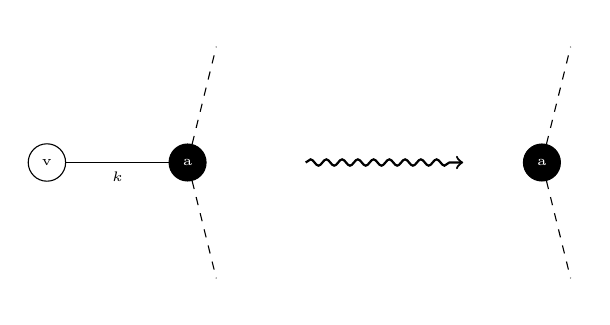
\begin{tikzpicture}[auto, node distance=1.3 cm]
      % Pre
      \begin{scope}[shift={(-0.5,0)}]
        \node[terminal] (a) at (0, 0) {a};
        \node[steiner] (b) [left=of a] {v};
        \node (sg) [above right = 1.3 and 0.1 of a] {};
        \node (sg2) [below right= 1.3 and 0.1 of a] {};

        %Edges
        \draw (a) edge node {$k$} (b);
        \draw[dashed] (a) to (sg);
        \draw[dashed] (a) to (sg2);
      \end{scope}

      \draw [->,decorate, thick,
      decoration={snake,amplitude=.4mm,segment length=2mm,post length=1mm}]
      (1.0,0) -- (3,0);
      % Post      
      \begin{scope}[shift={(4cm, 0)}]

        \node[terminal] (a) at (0, 0) {a};
        \node (sg) [above right = 1.3 and 0.1 of a] {};
        \node (sg2) [below right= 1.3 and 0.1 of a] {};

        %Edges
        \draw[dashed] (a) to (sg);
        \draw[dashed] (a) to (sg2);
      \end{scope}

  \end{tikzpicture}
  \caption{Removing a non-terminal with degree 1.}
  \label{fig:red:test:deg1}
\end{figure}

 While this reduction test is originally stated for the \gls{stp} \citep{hwang1992steiner}, it is also applicable to the \gls{pcstp}. Figure (\ref{fig:red:test:deg1})
  shows an example of removing a degree 1 non-terminal.

  \subsubsection{Non-Terminals of Degree 2 (NTD2)}
    \label{fig:red:test2}
\todo{These two sections probably use too different methods in defining their reductions}
    Similarly, let $G = (V,E,c,p)$ be an instance of the \gls{pcstp}, let $v \in G$ be a non-terminal with degree $|\delta(v)| = 2$, and let
    $u$ and $w$ be the two vertices adjacent to $v$. Then we can obtain a reduced, equivalent graph,
    $$G' = (V', E', c', p)$$
    where
    $$V' = V - v \mathnormal{,}$$
    $$E' = (E \setminus \{(u,v),(w,v)\}) \cup \{(u,w)\}\mathnormal{,}$$
    and
    $$c_{uw} =
    \begin{cases}
      \min(c_{uw}, c_{uv} + c_{vw}) & (u,w) \in E\mathnormal{,} \\
      c_{uv} + c_{vw} & \text{otherwise.}
    \end{cases}$$

    In other words, if $c_{uv} + c_{vw} <  c_{uw}$ then $(u,w)$ is redundant, can be removed, and $v$ and its edges
    can be contracted to a single edge.
    Otherwise $v$ and its edges are redundant and can be removed. Figure (\ref{fig:pre:ntd2})
    shows an example this reduction test.

\begin{figure}[h!]\centering
    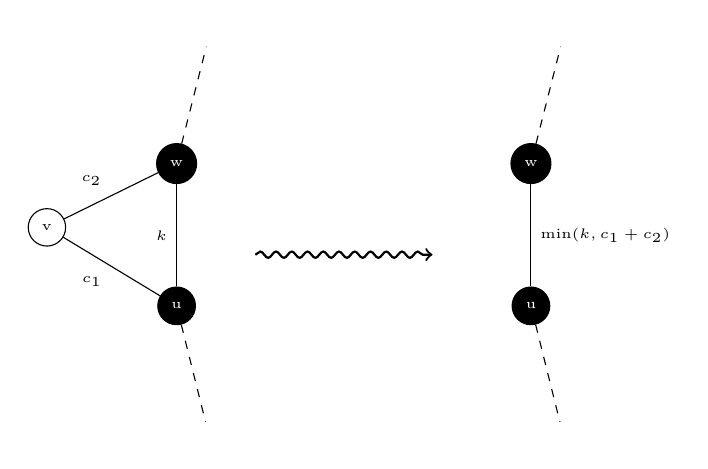
\begin{tikzpicture}[auto, node distance=1.3 cm]
      % Pre
      \begin{scope}
        \node[terminal] (a) at (0, -0.65) {u};
        \node[terminal] (b) [above=of a] {w};
        \node[steiner] (c) [above left= 0.65 and 1.3 of a] {v};
        \node (sg) [above right = 1.3 and 0.1 of b] {};
        \node (sg2) [below right= 1.3 and 0.1 of a] {};

        %Edges
        \draw (a) edge node {$k$} (b);
        \draw (a) edge node {$c_1$} (c);
        \draw (b) edge node[swap] {$c_2$} (c);
        \draw[dashed] (b) to (sg);
        \draw[dashed] (a) to (sg2);
      \end{scope}

      \draw [->,decorate, thick,
      decoration={snake,amplitude=.4mm,segment length=2mm,post length=1mm}]
      (1,0) -- (3.25,0);
      % Post      
      \begin{scope}[shift={(4.5cm, 0)}]
        \node[terminal] (a) at (0, -0.65) {u};
        \node[terminal] (b) [above=of a] {w};
        \node (sg) [above right = 1.3 and 0.1 of b] {};
        \node (sg2) [below right= 1.3 and 0.1 of a] {};

        %Edges
        \draw (a) edge node[swap] {$\min(k, c_1 + c_2)$} (b);
        \draw[dashed] (b) to (sg);
        \draw[dashed] (a) to (sg2);
      \end{scope}

  \end{tikzpicture}
  \caption{Removing a non-terminal with degree 2.}
  \label{fig:pre:ntd2}
\end{figure}

This test is another example of a reduction test for the \gls{stp} which can by directly applied to
 the \gls{pcstp}.
 \subsubsection{Terminals of Degree 1 (TD1)}\label{sec:pre:td1}
 When we have a terminal, $u$, of degree one, we can make the following two observations:
 \begin{enumerate}
 \item If the cost of the edge adjacent to $u$ is higher than $p_u$, then that edge is redundant, and
 \item additionally, if there exists a vertex with at least as high prize as $u$, then $u$ is redundant.
 \end{enumerate}
 These observations were stated first in \cite{uchoa2006reduction} -- however without the second condition,
 making the redundancy of $u$ potentially invalid -- and later corrected in \cite{rehfeldt2016reduction} as a combined test.

 We state here only the first part here as the TD1 test to allow for the disconnection of vertices with maximal prize.
 \begin{theorem}[Terminals of Degree 1 Test]
   Let $u$ be a terminal in $G$ with degree of 1 with adjacent edge $(u, v)$. If
   $p_u < c_{uv}$ then $(u,v)$ is redundant.
 \end{theorem}

 Applying this definition of TD1 in conjection with the UDV test (defined in Section \ref{sec:pre:udv})
 allows for the potential removal of terminals of degree one (see Figure \ref{fig:red:test:deg1}), giving the
  test defined in \cite{uchoa2006reduction} and \cite{rehfeldt2016reduction}.

\begin{figure}[h!]\centering
    \begin{tikzpicture}[auto, node distance=1.3 cm]
      % Pre
      \begin{scope}[shift={(-4,0)}]
        \node[terminal, label={$p_a$}] (a) at (0, 0) {v};
        \node[terminal, label={$p_v$}] (b) [left=of a] {u};
        \node (sg) [above right = 1.3 and 0.1 of a] {};
        \node (sg2) [below right= 1.3 and 0.1 of a] {};

        %Edges
        \draw (a) edge node {$k$} (b);
        \draw[dashed] (a) to (sg);
        \draw[dashed] (a) to (sg2);
      \end{scope}

      \draw [->,decorate, thick,
      decoration={snake,amplitude=.4mm,segment length=2mm,post length=1mm}]
      (-3,1) -- node [above=1mm,midway,text width=3cm, sloped, align=center] {$k\geq p_v$}
      (-1,2.3);
      \draw [->,decorate, thick,
      decoration={snake,amplitude=.4mm,segment length=2mm,post length=1mm}]
      (-3,-1) -- node [above=1mm,midway,text width=3cm, sloped, align=center] {$k < p_v$}
      (-1,-2.3);

      % Post      

      \begin{scope}[shift={(1.5cm, 0)}]

        \begin{scope}[shift={(0, 3cm)}]
          
          \node[terminal, label=right:{$p_a$}] (a) at (0, 0) {v};
          \node[terminal, label={$p_v$}] (b) [left=of a] {u};
        
          \node (sg) [above right = 1.3 and 0.1 of a] {};
          \node (sg2) [below right= 1.3 and 0.1 of a] {};

          % Edges
          \draw[dashed] (a) to (sg);
          \draw[dashed] (a) to (sg2);
        \end{scope}


        % Post2      
        \begin{scope}[shift={(0, -3cm)}]
          \node[terminal, label=right:{$p_a + (p_v - k)$}] (a) at (0, 0) {v};
          \node[terminal, label={$p_v$}] (b) [left=of a] {u};
          
          \node (sg) [above right = 1.3 and 0.1 of a] {};
          \node (sg2) [below right= 1.3 and 0.1 of a] {};
          
          % Edges
          \draw[dashed] (a) to (sg);
          \draw[dashed] (a) to (sg2);
        \end{scope}
      \end{scope}

      \draw [->,decorate, thick,
      decoration={snake,amplitude=.4mm,segment length=2mm,post length=1mm}]
      (4,3) -- node [above=1mm,midway,text width=3cm, sloped, align=center] {$\exists p_u \geq p_v$}
      (5,3);

      \draw [->,decorate, thick,
      decoration={snake,amplitude=.4mm,segment length=2mm,post length=1mm}]
      (4,-3) -- node [above=1mm,midway,text width=3cm, sloped, align=center] {$\exists p_u \geq p_v$}
      (5,-3);

      \begin{scope}[shift={(6.5cm, 0)}]

        \begin{scope}[shift={(0, 3cm)}]
          
          \node[terminal, label=right:{$p_a$}] (a) at (0, 0) {v};
        
          \node (sg) [above right = 1.3 and 0.1 of a] {};
          \node (sg2) [below right= 1.3 and 0.1 of a] {};

          % Edges
          \draw[dashed] (a) to (sg);
          \draw[dashed] (a) to (sg2);
        \end{scope}


        % Post3      
        \begin{scope}[shift={(0, -3cm)}]
          \node[terminal, label=right:{$p_a + (p_v - k)$}] (a) at (0, 0) {v};
          
          \node (sg) [above right = 1.3 and 0.1 of a] {};
          \node (sg2) [below right= 1.3 and 0.1 of a] {};
          
          % Edges
          \draw[dashed] (a) to (sg);
          \draw[dashed] (a) to (sg2);
        \end{scope}
    \end{scope}

  \end{tikzpicture}
  
  \caption{Removing a terminal of degree 1 (TD1 + UDV).}
  \label{fig:red:test:deg1}
\end{figure}

\subsubsection{Terminals of Degree 2 (TD2)} 
Similarly to TD1, we can disconnect terminals with degree 2 where both edges have costs higher than the prize
 of the terminal. Formally we state this as,
 \begin{theorem}[Terminals of Degree 2 Test]
   Let $u$ be a vertex with degree 2, such that vertices $v$ and $w$ are adjacent to $u$. Suppose that
   $$p_u \leq \min(c_{uv}, c_{uw})$$
   then any optimal solution must \textit{either} contain both edges or neither.
   Thus it is valid to replace the edges $(u,v)$ and $(u,w)$ with a single edge $(w,v)$ with cost
   $$c_{wv} = c_{uv} + c_{uw} - p_u\mathnormal{.}$$
 \end{theorem}

\begin{figure}[h!]\centering
    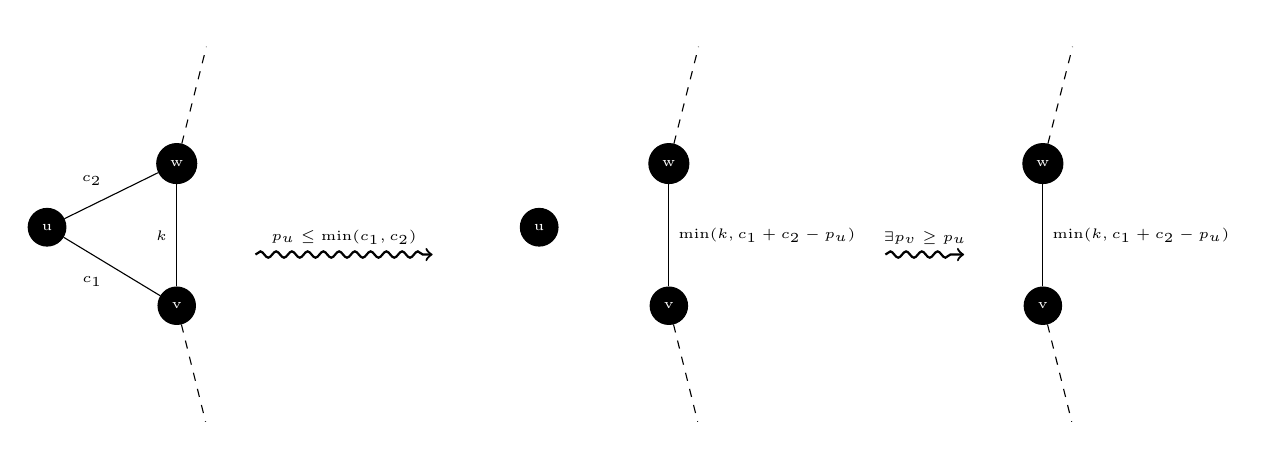
\begin{tikzpicture}[auto, node distance=1.3 cm]
      % Pre
      \begin{scope}
        \node[terminal] (a) at (0, -0.65) {v};
        \node[terminal] (b) [above=of a] {w};
        \node[terminal] (c) [above left= 0.65 and 1.3 of a] {u};
        \node (sg) [above right = 1.3 and 0.1 of b] {};
        \node (sg2) [below right= 1.3 and 0.1 of a] {};

        %Edges
        \draw (a) edge node {$k$} (b);
        \draw (a) edge node {$c_1$} (c);
        \draw (b) edge node[swap] {$c_2$} (c);
        \draw[dashed] (b) to (sg);
        \draw[dashed] (a) to (sg2);
      \end{scope}

      \draw [->,decorate, thick,
      decoration={snake,amplitude=.4mm,segment length=2mm,post length=1mm}]
      (1,0) -- node {$p_u \leq \min(c_1, c_2)$}
      (3.25,0);
      % Post      
      \begin{scope}[shift={(6.25cm, 0)}]
        \node[terminal] (a) at (0, -0.65) {v};
        \node[terminal] (b) [above=of a] {w};
        \node[terminal] (c) [above left= 0.65 and 1.3 of a] {u};
        \node (sg) [above right = 1.3 and 0.1 of b] {};
        \node (sg2) [below right= 1.3 and 0.1 of a] {};

        %Edges
        \draw (a) edge node[swap] {$\min(k, c_1 + c_2 - p_u)$} (b);
        \draw[dashed] (b) to (sg);
        \draw[dashed] (a) to (sg2);
      \end{scope}

      \draw [->,decorate, thick,
      decoration={snake,amplitude=.4mm,segment length=2mm,post length=1mm}]
      (9,0) -- node {$\exists p_v \geq p_u$}
      (10,0);

      \begin{scope}[shift={(11cm, 0)}]
        \node[terminal] (a) at (0, -0.65) {v};
        \node[terminal] (b) [above=of a] {w};
        \node (sg) [above right = 1.3 and 0.1 of b] {};
        \node (sg2) [below right= 1.3 and 0.1 of a] {};

        %Edges
        \draw (a) edge node[swap] {$\min(k, c_1 + c_2 - p_u)$} (b);
        \draw[dashed] (b) to (sg);
        \draw[dashed] (a) to (sg2);
      \end{scope}

  \end{tikzpicture}
  \caption{Removing a terminal with degree 2 (TD2 + UDV).}
  \label{fig:red:td2}
\end{figure}

\subsubsection{Unconnected Dominated Vertex (UDV)}\label{sec:pre:udv}
Proposed in \cite{rehfeldt2016reduction}, the \textit{unconnected dominated vertex test} reduces the
graph by removing any subgraph which contains at most one terminal which has less than maximum prize.
Stated formally as in the following theorem, which we will not prove.
\begin{theorem}[Unconnected Dominated Vertex Test]
  Consider a connected subgraph $S = (V_S, E_S, c, p)$ of $G$. Let $N_S = \{v \in V_s \mid p_v > 0\}$
  be the set of terminals in $S$. Then $S$ is redundant and removing it is valid if either
  \begin{enumerate}
  \item $N = \emptyset$, or
  \item $N = \{u\}$ and $p_u \leq \max_{v \in V \setminus \{u\}} p_v$.
  \end{enumerate}
\end{theorem}


This test can easily be applied as a special case for subgraphs consisting of a single,
 unconnected vertex.
 Figure (\ref{fig:red:test:deg1}) shows the application
 of TD1 followed directly by UDV.

\subsubsection{Minimum Adjacency (MA)}
Again defined in \cite{duin1989reduction} for the \gls{stp} but also applicable for the \gls{pcstp},
the \textit{minimum adjacency test}
(also known as the \textit{$V \setminus K$ test}) 
is a reduction test which contracts any adjacent
terminals which are connected by an edge with lower cost than either of their prizes.
 This is shown in Figure (\ref{fig:red:test:ma}).
 
\begin{figure}[h!]\centering
    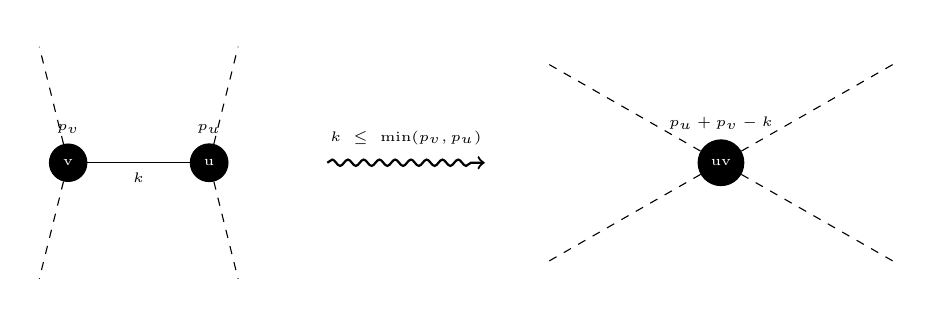
\begin{tikzpicture}[auto, node distance=1.3 cm]
      % Pre
      \begin{scope}[shift={(-0.5,0)}]
        \node[terminal, label={$p_u$}] (u) at (0, 0) {u};
        \node[terminal, label={$p_v$}] (v) [left=of u] {v};
        \node (sgu) [above right = 1.3 and 0.1 of u] {};
        \node (sgu2) [below right= 1.3 and 0.1 of u] {};

        \node (sgv) [above left = 1.3 and 0.1 of v] {};
        \node (sgv2) [below left= 1.3 and 0.1 of v] {};

        %Edges
        \draw (u) edge node {$k$} (v);
        \draw[dashed] (u) to (sgu);
        \draw[dashed] (u) to (sgu2);
        \draw[dashed] (v) to (sgv);
        \draw[dashed] (v) to (sgv2);
      \end{scope}

      \draw [->,decorate, thick,
      decoration={snake,amplitude=.4mm,segment length=2mm,post length=1mm}]
      (1.0,0) -- node [above=1mm,midway,text width=3cm, sloped, align=center] {$k \leq \min(p_v, p_u)$}
      (3,0);
      % Post      
      \begin{scope}[shift={(6cm, 0cm)}]
        \node[terminal, label={$p_u + p_v - k$}] (u) at (0, 0) {uv};
        \node (sgu) [above right = 1. and 2.0 of u] {};
        \node (sgu2) [below right= 1. and 2.0 of u] {};
        \node (sgv) [above left = 1. and 2.0 of u] {};
        \node (sgv2) [below left= 1. and 2.0 of u] {};

        %Edges
        \draw[dashed] (u) to (sgu);
        \draw[dashed] (u) to (sgu2);
        \draw[dashed] (u) to (sgv);
        \draw[dashed] (u) to (sgv2);
      \end{scope}

  \end{tikzpicture}
  \caption{Minimum adjacency test.}
  \label{fig:red:test:ma}
\end{figure}

\begin{theorem}[Minimum Adjacency]
  Let $u$ and $v$ be adjacent terminals in $G$. If we have
  $$c_{uv} \leq \min(p_u, p_v)$$
  and
  $$c_{uv} = \min_{(u, w) \in E}c_{uw}$$
  then it is valid to contract $u$ and $v$.
\end{theorem}
\begin{proof}
  It can be shown that any solution $T$ for the \gls{pcstp} problem defined by a graph $G$
  which contains $u$ but not $(u,v)$ can
  be transformed into a solution $T'$ which contains $(u,v)$ where $c(T') \leq c(T)$.

  \paragraph{Case 1: ($v \in V_T$)}
  Let $(u, w) \in E_T$ be the first edge in the simple path from $u$ to $v$. By assumption, we
  have that $c_{uv} \leq c_{uw}$, and the tree $T'$ constructed by removing $(u,w)$ from $T$ and
  adding $(u,v)$ has cost
  $$c(T') = c(T) - c_{uw} + c_{uv} \leq T\mathnormal{.}$$
  \paragraph{Case 2: ($v  \not\in V_T$)}
  Let $T'$ be the tree obtained by adding $(u,v)$ to $T$. As per the assumption that $\min(p_u, p_v) \geq c_{uv}$,
  we have that $T'$ has cost,
  $$c(T') = c(T) + c_{uv} - p_{uv} \leq c(T)\mathnormal{.}$$
\end{proof}


\subsection{Steiner Distance Reduction Tests}\label{sec:sd-red-test}
% $$d(u,v) = \min \{ c(P) \mid P \in \mathcal{P}_{uv}\}$$
More complex tests can be described in terms
of the concepts Steiner distance and Bottleneck distance. These were originally stated for
the \gls{stp} in, amongst others, \cite{duin1989edge,duin1989reduction} and later
adapted for the \gls{pcstp} in \cite{uchoa2006reduction}.

First we must make some definitions.
If $P = (..., u, ..., w, ...)$ is a simple path in $G$, then $P_{uw}$ is
the subpath in $P$ starting at vertex $u$ and ending in vertex $w$,
\todo{Some of this should probably go in a notations section}
that is $P_{u,w} = (u, ...,w)$. Then we define the \textit{Steiner distance} of
 $P_{uw}$ as,

 $$sd(P_{uw}) = \sum_{(i,j) \in E(P_{u,w})} c_{i,j} -
 \sum_{v \in V(P) \setminus \{u,w\}} p_{v}\mathnormal{.}$$
 We then denote the Steiner distance of a simple path, $P$, as the maximal Steiner
 distance found among subpaths of $P$,
 $$sd(P) = \max_{u,w \in P} sd(P_{uw})\mathnormal{.}$$
 Let $\mathcal{P}_{uw}$ be the set of all simple paths
 connecting vertices $u$ and $w$ in
 $G$, then we denote the \textit{bottleneck distance} between $u$ and $w$ as the minimal Steiner
  distance among paths in $\mathcal{P}_{uw}$,
  $$B(u,w) = \min_{P \in  \mathcal{P}_{uw}} sd(P)\mathnormal{.}$$
  The bottleneck distance is a measure of the worst case \textit{additional cost}
  \todo{Proof? Maybe.}
 of connecting
 two disjoint subgraphs containing vertices $u$ and $v$ respectively in $G$.

  \missingfigure{Some visual intuition on the bottleneck distance}

  Finally, we denote the bottleneck distance between vertices $u$ and $w$ \textit{excluding}
  the edge $e$ as,
  $$B(u,w)^{-e} = \min_{P \in  \mathcal{P}_{uw}, e \not \in P} sd(P)\mathnormal{.}$$


 \cite{uchoa2006reduction} shows that calculating the bottleneck distance
 is an NP hard problem by reduction from the Hamiltonian Path problem. Hence,
 exactly calculating the bottleneck distance is infeasible. However, \cite{uchoa2006reduction}
 also claims that existing heuristics are fast and give strong upper bounds.

It is worth noting that due to
\begin{enumerate*}[label={\alph*)}]
\item the relatively new proposal of the Steiner/bottleneck distances in \cite{uchoa2006reduction} for the \gls{pcstp}, and
\item their computational complexities,
\end{enumerate*}
the reduction tests stated in this section have been applied in literature
using ordinary distance (i.e. ignoring prizes) and shortests paths
instead of the Steiner and bottleneck distances. This corresponds to the direct application of
reduction tests
proposed for the \gls{stp} in \cite{duin1989edge,duin1989reduction}. Since this results in
upper bounds on the bottleneck distance, the original
tests are still valid for the \gls{pcstp},
but are weaker than the natively tests proposed in \cite{uchoa2006reduction}.

When we talk
 about \textit{shortest path relaxations} of the following tests, this is what we are referring to.

 \subsubsection{Special Distance (SD)}
 \label{sec:red:test:sd}
 Using the \gls{pcstp} version of the Steiner and bottleneck distances, \cite{uchoa2006reduction} proves
  the validity of the more general \textit{special distance test}.
 \begin{theorem}[Special Distance Test]
 Consider any edge $(u,v) \in E$. If we have
 $$B(u,v)^{-(u,v)} \leq c_{uv}$$
 then $(u,v)$ is redundant.
\end{theorem}
 \begin{proof}
   Let $T  \subseteq G$ be an optimal solution to the \gls{pcstp} in graph $G$
   where we have
   $$B(u,v)^{-(u,v)} \leq c_{uv}$$
   for some edge $(u,v) \in E_T$, and let $(T_1, T_2)$ be the cut bridged
   by $(u,v)$.

   Consider then the simple path $P \in \mathcal{P}_{uv}$ from $u$ to $v$ which doesn't
    contain $(u,v)$ and has
   $$sd(P) = B(u,v)^{-(u,v)}\mathnormal{.}$$

   Since $T$ is a tree, and $P$ by definition doesn't contain the edge $(u,v)$
   then we must have that $P$ consists of a subpath contained in $T_1$, followed by
   a subpath not contained in $T$, followed by a subpath contained in $T_2$.
   In other words, we have,
   $$P = (u, P_1, w, P_2, z, P_3, v)$$
   as shown in Figure \ref{fig:red:test:sd:thm}.

   Then by definition we have,
   $$sd(P_2) \leq sd(P) = B(u,v)^{-(u,v)} \leq c_{uv}$$
   and we construct another solution $T'$ by replacing $(u,v)$ with the
   vertices and edges in $P_2$ which has cost
   $$c(T') = c(T) - c_{uv} + sd(P_2) \leq c(T)\mathnormal{.}$$
   Hence $T'$ also optimal in $G$ and $(u,v)$ is by definition redundant.
\end{proof}
\begin{figure}[h!]\centering
    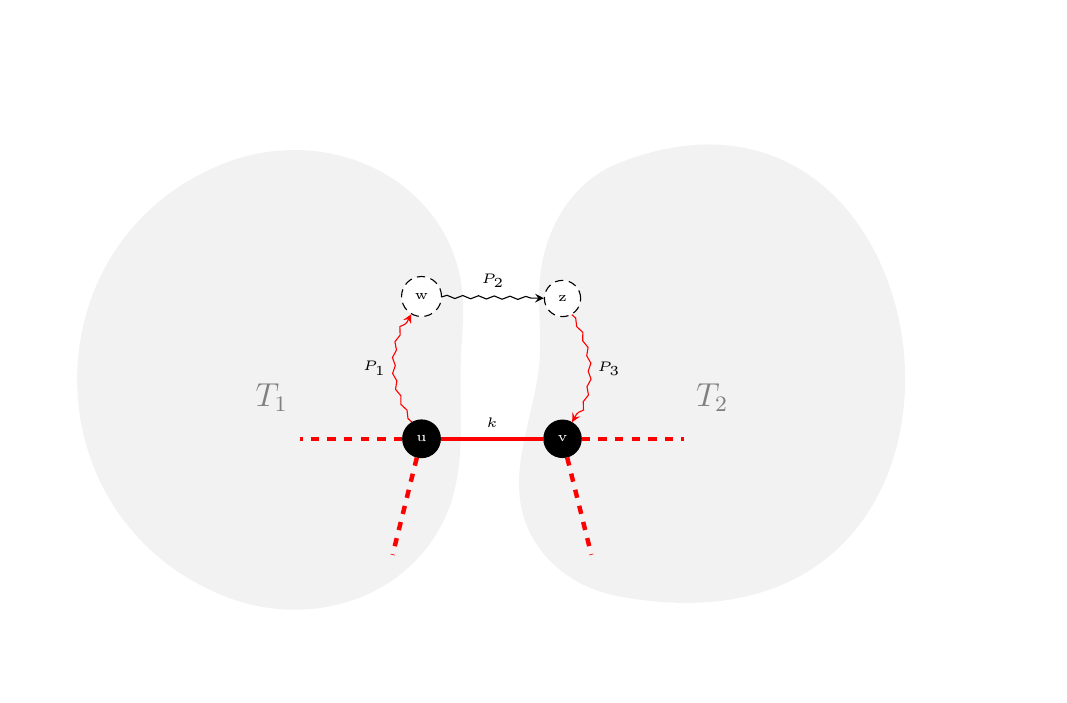
\begin{tikzpicture}[auto, node distance=1.3 cm]
      % Pre
      \begin{scope}[]
        \path[fill=black!5,use Hobby shortcut,closed=true]
        (-2.5, -2) .. (0.3,-1) .. (.5,1) .. (.5,2)  .. (-2.5,3.5);
        \path[fill=black!5,use Hobby shortcut,closed=true]
        (2.5, -2) .. (1.3,-1) .. (1.5,1) .. (1.5,2)  .. (2.5,3.5);

        \node[terminal] (u) at(0, 0) {u};
        \node[subgraph, above left= 0.05cm and 1.4cm of u] {$T_1$};
        \node[steiner, densely dashed] (w1) [above=of u] {w};
        
        \node[terminal] (v) [right= of u] {v};
        \node[subgraph,above right= 0.05 and 1.4cm  of v] {$T_2$};
        \node[steiner, densely dashed] (w2) [above=of v] {z};
        \node (sga) [left= of u] {};
        \node (sga2) [below left= 1.3 and 0.1 of u] {};

        \node (sgb) [right=  of v] {};
        \node (sgb2) [below right= 1.3 and 0.1 of v] {};

        
        
        %Edges
        \draw[selected] (u) edge node {$k$} (v);
        \draw[dashed, selected] (u) to (sga);
        \draw[dashed, selected] (u) to (sga2);

        \draw[dashed, selected] (v) to (sgb);
        \draw[dashed, selected] (v) to (sgb2);

        \draw (u) edge[snake it, red, bend left] node[text=black] {$P_1$} (w1);
        \draw (w1) edge[snake it] node {$P_2$} (w2);
        \draw (w2) edge[snake it, red, bend left] node[text=black] {$P_3$} (v);
      \end{scope}

      % \draw [->,decorate, thick,
      % decoration={snake,amplitude=.4mm,segment length=2mm,post length=1mm}]
      % (4,0) -- node [above=1mm,midway,text width=3cm, sloped, align=center] {}
      % (6,0);
      % Post      

  \end{tikzpicture}
  \caption{The optimal solution, $T = T_1 \cup T_2$ connected by $(u,v)$.
    Since $c(u,v) \geq B(u,v)^{-(u,v)}$,
  the simple path $P_2$ has cost no larger than $(u,v)$ and can replace it in $T$.}
  \label{fig:red:test:sd:thm}
\end{figure}

\subsubsection{Non-Terminals of Degree 3 (NTD3)}
\label{sec:red:test:deg3}
Another bottleneck distance based test,
also proved valid for the \gls{pcstp} in \cite{uchoa2006reduction},
is the \textit{non-terminals of degree 3 test}.
\begin{theorem}[Non-Terminals of Degree 3 Test]\label{thm:ntd3}
  Let $u$ be a vertex with degree 3 in $G = (V, E, c, p)$,
  and let $v$, $w$, and $z$ be its adjacent
  vertices. If we have
  $$\min\left(B(v,w) + B(v,z), B(w,v) + B(w,z),  B(z, v)+ B(z, w)\right) \leq
  c_{uv} + c_{uw} + c_{uz}$$
  then there exists an optimal solution to $G$ where $u$ has degree of
  \textit{at most} 2, that is $|\delta(u)| \leq 2$. Thus $u$ and its three edges, can be replaced by
  the edges $\{(v, w), (w,z), (z,v)\}$ with costs
  $$c_{vw} = c_{vu} + c_{uw},\quad c_{wz} = c_{wu} + c_{uz},\quad c_{zv} = c_{zu} + c_{uv}\mathnormal{.}$$
\end{theorem}
\begin{proof}   
  W.l.o.g. consider the case where $B(v,w) + B(v,z) \leq c_{uv} + c_{uw} + c_{uz}$,
  and let $T$ be an optimal solution which contains $(u,v)$, $(u,w)$, and $(u,z)$.

  Let $P_1 = (v, ..., w)$ be the simple path with Steiner distance
  $$sd(P_1) = B(v,w)$$
  and similarly let $P_2 = (v, ..., z)$ be the simple path with Steiner distance
  $$sd(P_2) = B(v,z)\mathnormal{.}$$
  This gives us the situation in Figure (\ref{fig:red:test:ntd3:thm}). Note that $u$ may be a part of either paths.

  Let $T_v$, $T_w$, and $T_z$ be the subtrees of $T$ obtained by
  removing the edges adjacent to $u$ from $T$, and construct a new solution with
   total cost no-larger than $T$ as,
   $$T' = T_v \cup T_w \cup T_z \cup P_1 \cup P_2\mathnormal{.}$$
   We must have $|\delta_{T'}(u)| \leq 2$. If we had $|\delta_{T'}| = 3$ then
   we would have
   $$P_1 = \left[v, (v,u), u, (u,w), w \right]$$
   and
   $$P_2 = \left[v, (v,u), u, (u,z) z \right]$$
   giving us
   $$B(v,w) + B(v, z) = sd(P_1) + sd(P_2) = 2 c_{vu} + c_{uw} + c_{uz} > c_{vu} + c_{uw} + c_{uz}$$
   which is a contradiction to our original assumption that
   $$B(v,w) + B(v,z) \leq c_{uv} + c_{uw} + c_{uz}\mathnormal{.}$$
   Thus $T'$ is an optimal solution to $G$ with $|\delta_{T'}(u)| \leq 2$.
\end{proof}
\begin{figure}[h!]\centering
    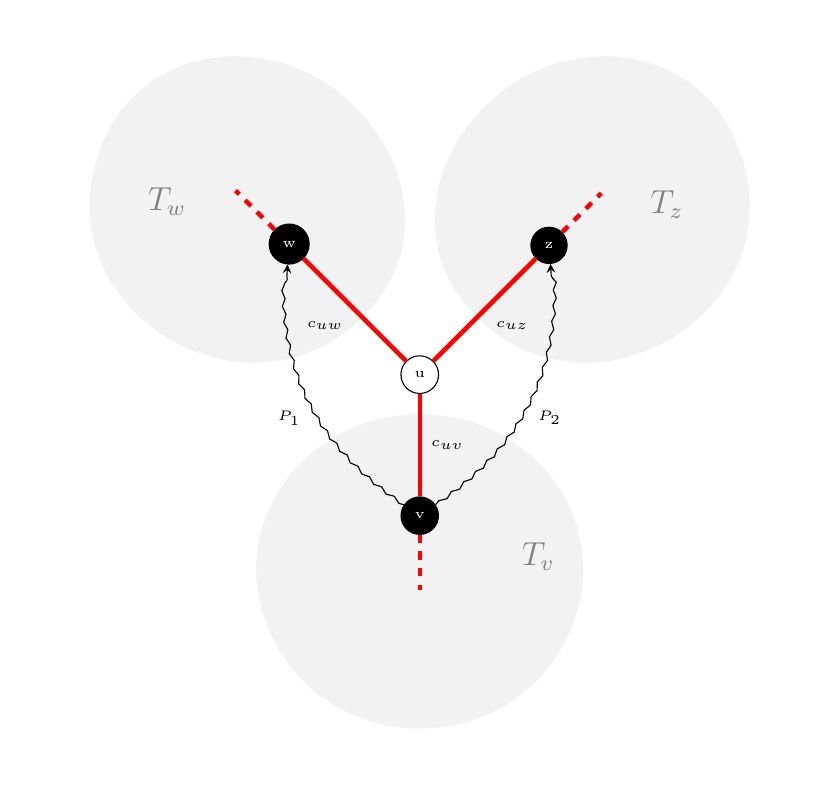
\begin{tikzpicture}[auto, node distance=1.3 cm]
      % Pre
      \begin{scope}[]
        \path[fill=black!5,use Hobby shortcut,closed=true]
        (-0.5, 1) .. (-4, 3) .. (-0.5,3);
        \path[fill=black!5,use Hobby shortcut,closed=true]
        (.5, 1) .. (4,3) .. (.5,3);
        \path[fill=black!5,use Hobby shortcut,closed=true]
        (0, -.5) .. (-2,-3) .. (2,-3);

        \node[steiner] (u) at(0, 0) {u};
        \node[terminal] (w) [above left=1.3 and 1.3 of u] {w};
        \node[terminal] (v) [below= of u] {v};
        \node[terminal] (z) [above right= 1.3 and 1.3 of u] {z};

        \node[subgraph, above left= 0.05cm and 1 cm of w] {$T_w$};
        \node[subgraph,above right= 0.05cm and 1 cm of z] {$T_z$};
        \node[subgraph, below right= 0.05cm and 1 cm of v] {$T_v$};
        
        \node (sgw) [above left= 0.7 of w] {};
        \node (sgv) [below= 0.7 of v] {};
        \node (sgz) [above right = 0.7 of z] {};
        
        %Edges
        \draw[selected] (u) edge node {$c_{uv}$} (v);
        \draw[selected] (u) edge node {$c_{uw}$} (w);
        \draw[selected] (u) edge node[swap] {$c_{uz}$} (z);
        \draw[dashed, selected] (v) to (sgv);
        \draw[dashed, selected] (w) to (sgw);
        \draw[dashed, selected] (z) to (sgz);

        \draw (v) edge[snake it, bend left] node[text=black] {$P_1$} (w);
        \draw (v) edge[snake it, bend right] node[swap,text=black] {$P_2$} (z);
      \end{scope}

      % \draw [->,decorate, thick,
      % decoration={snake,amplitude=.4mm,segment length=2mm,post length=1mm}]
      % (4,0) -- node [above=1mm,midway,text width=3cm, sloped, align=center] {}
      % (6,0);
      % Post      

  \end{tikzpicture}
  \caption{Non-Terminal of $|\delta(u)| = 3$ which connects the subtrees $T_v$, $T_w$, and $T_z$. The simple paths $P_1$ and $P_2$ provide an
     alternate way of reconnecting $T$ with at least as good cost.}
  \label{fig:red:test:ntd3:thm}
\end{figure}

\subsubsection{Non-Terminals of Degree k (NTDk)}
\todo[inline]{This is stated somewhat in the Uchoa paper and weirdly in the Rehfeldt paper. The latter claims that the former proves it, but there is no such proof. Shouldn't be too difficult}

\subsection{Voronoi Reductions}

Reduction test based on a Voronoi decomposition of the input graph was introduced for the \gls{pcstp} by \cite{rehfeldt2016reduction}. These reduction tests broadly
involve using the Voronoi decomposition to generate conditional lower bounds based on vertex inclusion/exclusion. Given a strong upper bound, these can be used
to reduce the graph.

\paragraph{Voronoi Decomposition of a \gls{pcstp} Graph}

Given an instance of the \gls{pcstp} with the undirected graph $G = (V, E, c, p)$ and terminal set
$N \subseteq V$, we define a Voronoi region for a given terminal, $i \in N$, as the set of nonterminals
which are closer to $i$ than any other terminal in terms of simple shortests paths -- that is,
$$R_i = \left\{v \in V \setminus N \mid i = \argmin_{u \in N} d_{vu}\right\}$$
where $R_i$ is the Voronoi region covered by the terminal $i$ and $d_{vu}$ is the shortest path between vertices
$v$ and $u$.

We then define the \textit{radius} of the $i$th Voronoi region as the shortest path from its centre (the $i$ith terminal)
to any vertex not in the region,
$$\radius(i) = \min_{v \not\in R_i} d_{iv}\mathnormal{.}$$
From this we define a \textit{prize-collecting radius} of a region as,
$$\pcradius(i) = \min(\radius(i), p_i)\mathnormal{.}$$
We note that we can intuitively see the \textit{pc radius} of a region as a kind of lower bound
on the cost contribution
 of that region to any
 \textit{connected}, multi-vertex solution. Either the prize for the respective terminal must be paid as a penalty
 \textit{or} the terminal must be connected to the rest of the tree by a path which must have some cost \textit{higher}
 than the \textit{radius} of the region.

 Finally, let
 $$z_1, z_2, ..., z_{|N|}$$
 be a monotonically increasing ordering of terminals such that
$$\pcradius(z_1) \leq \pcradius(z_2) \leq ... \leq \pcradius(z_{|N|})\mathnormal{.}$$

\paragraph{Lower Bound Reductions}

The first reduction we can present based on Voronoi regions is based on a lower bound given that some nonterminal is
part of a solution. This was first introduced for the \gls{stp} by \citet{polzin2001improved} and later adapted by
\citet{rehfeldt2016reduction} for the \gls{pcstp}.

\begin{theorem}\label{thm:vor:1}
  Let $T = (V_T, E_T, c, p)$ be a solution to the \gls{pcstp} in the graph $G = (V, E, c, p)$ with terminal set $N$ such that
  $v_k \in V_T$ for some $v_k \in V \setminus N$. Finally, let $v_a \in N$ and $v_b \in N$ be the two terminals \textit{closest}
  to $v_k$, then we have
  $$d(v_a, v_k) + d(v_b, v_k) + \sum_{i = 1}^{|N| - 2} \pcradius(z_i) \leq c(T)\mathnormal{.}$$
\end{theorem}
\begin{proof}
  Consider a solution $T$ as described above containing some nonterminal $u \in V_T$.
  For all $j \in (N \cap V_T)$ let $P_i$ be the
  path from $v_i$ to $u$ in $T$ (this must be well defined as $T$ is a tree). Furthermore,
  let $P_i'$ be the subpath of $P_i$ which starts in $v_i$ and ends in the first vertex along
  $P_i$ not in $R_i$, and
  let $\Delta(P_i)$ be the number of times a Voronoi border is crossed by the path $P_i$ and
  let $\Delta(P_i) = \infty$ if $v_i \not\in V_T$.

  Let $v_m$ and $v_l$ be two terminals such that $\Delta(P_m) + \Delta(P_l)$ is minimal among
  all pairs of terminals where $P_m$ and $P_l$ are disjoint paths. Since $T$ is a tree and
  $v_i$ must have degree of at least $2$ (See Section \ref{sec:red:test:deg1}) there must
  be at least one such pair.

  Consider the set of paths
  $$\mathcal{P} = \{P_i' \mid i \in (V_T \cap N) \setminus \{v_m, v_l\} \}
  \mathnormal{.}$$
  These paths must be disjoint as $T$ contains no cycles. The paths in $\mathcal{P}$
  alongside $P_m$ and $P_l$ are then all pairwise disjoint paths which cover a subset of the
  edges
  in $E_T$.

 \begin{figure}[h!]
     \centering
     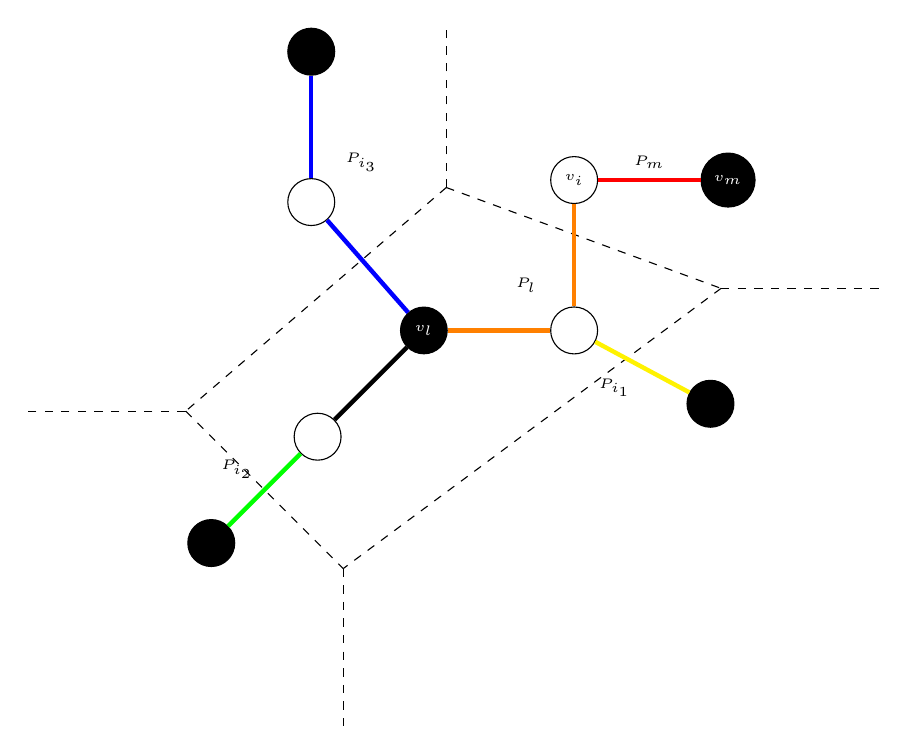
\begin{tikzpicture}[auto, node distance=1.3cm]
       \node[steiner] (vi) {$v_i$};
       \node[steiner] (vib) [below= of vi] {$\phantom{v_i}$};

       \node[terminal] (vj) [right= of vi] {$v_m$};
       \node[terminal] (vl) [left= of vib] {$v_l$};
       \node [above left= 0.2 of vib] {$P_l$};

       
       \node[steiner]  (vlal) [above left= 1.2 and 1 of vl] {$\phantom{v_i}$};
       \node [above right= 0.05 and 0.1 of vlal] {$P_{i_3}$};
       \node[terminal]  (vlala) [above= of vlal] {$\phantom{v_i}$};

    \node[steiner] (vll) [below left=  of vl] {$\phantom{v_i}$};
    \node[terminal] (vlll) [below left=  of vll] {$\phantom{v_i}$};

    \node[terminal] (vibr) [below right= 0.5 and 1.3 of vib] {$\phantom{v_i}$};

    \begin{scope}
      % VORONOI :(
            \draw[dashed] let \p1=(vll),\p2=(vlll) in 
            ({(\x1+\x2)/2-1cm},{(\y1+\y2)/2+1cm}) coordinate(A)
            --
            ({(\x1+\x2)/2+1cm},{(\y1+\y2)/2-1cm}) coordinate(AA);
            \draw[dashed] let \p1=(vl),\p2=(vlal) in 
            ({(\x1+\x2)/2+1cm},{(\y1+\y2)/2+1cm}) coordinate(B)
            --
            (A);

            \draw[dashed] let \p1=(vib),\p2=(vibr) in 
            ({(\x1+\x2)/2+1cm},{(\y1+\y2)/2+1cm}) coordinate(C)
            --
            (AA);

            \draw[dashed] (B) -- (C);
            \draw[dashed] (C) -- ([xshift=2cm]C);
            \draw[dashed] (B) -- ([yshift=2cm]B);
            \draw[dashed] (AA) -- ([yshift=-2cm]AA);
            \draw[dashed] (A) -- ([xshift=-2cm]A);
   \end{scope}
   \begin{scope}
     % Edges
     \draw[selected, blue] (vlala) edge (vlal);
     \draw[selected, blue] (vlal) edge (vl);

     \draw[selected, green] (vlll) edge node[black] {$P_{i_2}$} (vll);
     \draw[selected, yellow] (vibr) edge node[black] {$P_{i_1}$} (vib);

     \draw[selected, black] (vll) edge (vl);
     
     \draw[selected] (vj) edge node[above] {$P_m$} (vi);

     \draw[selected, orange] (vl) edge (vib);
     \draw[selected, orange] (vib) edge (vi);
   \end{scope}
  \end{tikzpicture}
  
  \caption{Example solution of the \gls{pcstp} split into paths.}
  \label{fig:pre:vor:pro}
\end{figure}
  

An example of this partition of $T$ is shown in Figure (\ref{fig:pre:vor:pro}). The two ``closest''
terminals $v_l$ and $v_m$ have disjoint paths $P_l$ and $P_m$ to the interesting nonterminal $v_i$.
The rest of the solution is partitioned by $P_i'$ paths, these paths run from a terminal towards $v_i$
until -- and inclusive -- the first edge which crosses a Voronoi boundary. No two paths in such a decomposition
can share an edge. This follows directly from the facts that each Voronoi region contains
\textit{only} a single terminal, and that there can be only a single path from vertex to $v_i$ (no cycles).
Hence a border edge can only be crossed in one ``direction'' this way.

With this, clearly the total edge costs of these paths cannot be greater than the edge cost of $T$. We select only
 in this way a subset of the edges of $T$, and never select an edge twice. In other words, we have
  \begin{equation}
    c(E(P_m)) + c(E(P_l)) + \sum_{P_i \in \mathcal{P}} c(E(P)) \leq c(E_T)\mathnormal{.}\label{eq:vor:one}
  \end{equation}

  
  Additionally, by definition
  we must have that $P_i' \leq \pcradius(i)$, $d(v_m, v_i) \leq c(E(P_m))$, and
  $d(v_l, v_i) \leq c(E(P_l))$. This gives us

  \begin{equation}
d(v_l, v_i) + d(v_m, v_i) + \sum_{P_i \in \mathcal{P}} \pcradius(i) \leq c(E(P_m)) + c(E(P_l)) + \sum_{P_i \in \mathcal{P}} c(E(P))\label{eq:vor:two}
\end{equation}


  Finally, for the set of terminals not covered by $T$, we must -- again by the definition of $\pcradius$ -- have
  \begin{equation}
  \sum_{i \in N \setminus V_T} \pcradius(i) \leq \sum_{i \in N \setminus V_T} p_i \mathnormal{.}\label{eq:vor:three}
  \end{equation}

  By combining the equations (\ref{eq:vor:one}), (\ref{eq:vor:two}), and (\ref{eq:vor:three}), and
   by the definition of vertices $v_a$ and $v_b$ being the terminals closest to $v_i$ we have,
   $$d(v_a, v_k) + d(v_b, v_k) + \sum_{i = 1}^{|N| - 2} \pcradius(z_i) \leq c(T)$$
   and we are done.
 \end{proof}
 If a nonterminal is found such that the bound in Theorem \ref{thm:vor:1} is larger than the objective value of
 any found feasible solution, then that nonterminal is redundant and it is valid to remove it and its edges.

 Similar 
\begin{theorem}\label{thm:vor:2}
  Let $T = (V_T, E_T, c, p)$ be a solution to the \gls{pcstp} in the graph $G = (V, E, c, p)$ with terminal set $N$ such that
  $v_k \in V_T$ for some $v_k \in N$ and $V_T \neq \{v_k\}$. Finally, let $v_b \in N$ be the terminal \textit{closest}
  to $v_k$, and let $z'_1, ..., z_{|N|-1}$ be an ordering of the set $N \setminus \{v_k\}$ such that
  $$\pcradius(z_1) \leq ... \leq \pcradius(i) \leq ... \leq \pcradius(z'_{|N|-1})$$
  then we have
  $$d(v_b, v_k) + \sum_{i = 1}^{|N| - 2} \pcradius(z'_i) \leq c(T)\mathnormal{.}$$
\end{theorem}
The proof of Theorem \ref{thm:vor:2} is symmetric to the proof of Theorem \ref{thm:vor:1}. If a terminal is found such that
the respective lower bound is higher than the objective value of a given incumbent, then the terminal is redundant and it is
 valid to remove it from $G$ along with its adjacent edges.

 \subsection{Summary of Usage}\label{sec:pre:summary-usage}
There's a general consensus in literature that preprocessing is an important part of producing solutions
for the \gls{pcstp}. Preprocessing described in this section is applied natively to the \gls{pcstp}
in all of
\cite{lucena2004strong, Ljubic:2004:memetic, ljubic2005solving,akhmedov2016divide,gamrath2017scip}.
Additionally, preprocessing is applied to the \gls{sap} in \cite{leitner2016dual}, and proposed
as further improvements in \cite{fu2014knowledge}.

\paragraph{Combinations of Tests}

In \cite{lucena2004strong} all four of the degree tests (NTD1, NTD2, TD1+UDV, TD2+UDV) are
applied alongside shortest path relaxations of SD and NTDk (for ``small'' numbers of $k$)
tests. They do not
present in which order tests are applied or how often they are repeated, but they
do present the graph sizes of their benchmark cases before and after applying preprocessing.

\cite{Ljubic:2004:memetic} and \cite{ljubic2005solving} share a preprocessing routine
 which applies in order:
\begin{enumerate}
\item degree one tests: NTD1+TD1+UDV,
\item degree two tests: NTD2+TD2.
\item shortest path relaxation of the special distance test (here called the least cost test),
\item shortest path relaxation of NTDk for $k = 3,...,8$, and
\item the minimum adjacency test.
\end{enumerate}
until a fixpoint is reached. They present both numbers on graph reduction and preprocessing
time. Across all problem instances, they report on average
a 45\% reduction in graph size.

\cite{akhmedov2016divide} applies the four degree tests until a fixpoint is reached. They
report reduction in graph sizes for their test cases as well as pre-processing time and
total computation time with/without preprocessing.

\todo[inline]{Maybe insert a comparison of computational experiences (table)}

\begin{example}
Finally, we'll give an example of the power of
these preprocessing methods. Figure \ref{fig:pre:ex} shows how just
the local tests defined in Section \ref{sec:pre:local} are enough
to solve the -- admittedly simplistic -- instance of the \gls{pcstp}
from Figure \ref{fig:pcstp:01}.


\begin{figure}[h!]\centering
  \begin{tikzpicture}[auto,
    node/.style={minimum width=10cm, inner sep={(10cm, 5cm)}}]
    \node[minimum width=5cm,
      minimum height=2.5cm] (1) {
      \begin{tikzpicture}[node distance=1.5 cm,
            every node/.style={minimum width=0, minimum height=0}]]
    % Nodes
    \node[terminal, label={12}] (a) at (0,0) {a};
    \node[steiner] (b) [right=of a] {b};
    \node[steiner] (c) [right=of b] {c};
    \node[terminal, label={10}] (d) [above =of c] {d};
    \node[steiner] (e) [left=of d] {e};
    \node[steiner] (f) [left=of e] {f};
    \node[terminal, label={3}] (g) [above right=0.75 and 1.3 of c] {g};
    % Edges

    \draw (a) edge node[below]{4} (b);
    \draw (b) edge node[near start]{5} (d);
    \draw (b) edge node[below]{8} (c);
    \draw (c) edge node{3} (d);
    \draw (c) edge node{2} (g);
    \draw (c) edge node[near start]{5} (e);
    \draw (d) edge node {6} (e);
    \draw (d) edge node{10} (g);
    \draw (e) edge node{1} (f);
    \end{tikzpicture}
  };
  
  \node[minimum width=5cm,
      minimum height=2.5cm] (2) at (9, 0) {
    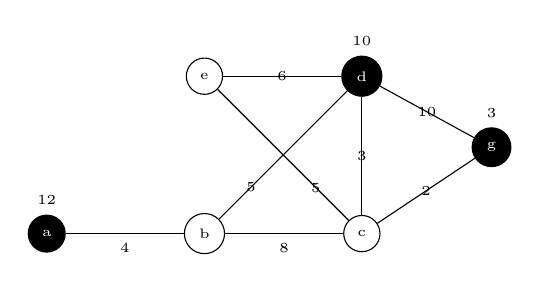
\begin{tikzpicture}[node distance=1.5 cm,
          every node/.style={minimum width=0, minimum height=0}]]
    % Nodes
    \node[terminal, label={12}] (a) at (0,0){a};
    \node[steiner] (b) [right=of a] {b};
    \node[steiner] (c) [right=of b] {c};
    \node[terminal, label={10}] (d) [above =of c] {d};
    \node[steiner] (e) [left=of d] {e};
    \node[terminal, label={3}] (g) [above right=0.75 and 1.3 of c] {g};
    % Edges

    \draw (a) edge node[below]{4} (b);
    \draw (b) edge node[near start]{5} (d);
    \draw (b) edge node[below]{8} (c);
    \draw (c) edge node{3} (d);
    \draw (c) edge node{2} (g);
    \draw (c) edge node[near start]{5} (e);
    \draw (d) edge node{6} (e);
    \draw (d) edge node{10} (g);
  \end{tikzpicture}
};

\node[minimum width=5cm,
      minimum height=2.5cm](3) at (0, -4) {
  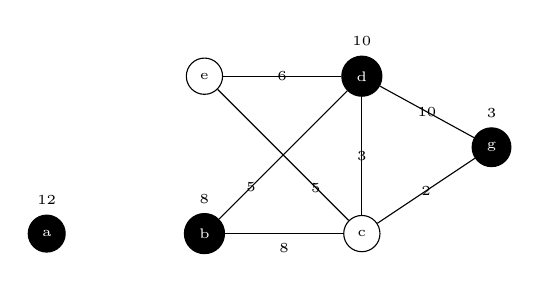
\begin{tikzpicture}[node distance=1.5 cm,
        every node/.style={minimum width=0, minimum height=0}]]
    % Nodes
    \node[terminal, label={12}] (a) at (0,0){a};

    \node[terminal] (b) [right=of a, label={8}] {b};
    \node[steiner] (c) [right=of b] {c};
    \node[terminal, label={10}] (d) [above =of c] {d};
    \node[steiner] (e) [left=of d] {e};
    \node[terminal, label={3}] (g) [above right=0.75 and 1.3 of c] {g};
    % Edges

    \draw (b) edge node[near start]{5} (d);
    \draw (b) edge node[below]{8} (c);
    \draw (c) edge node{3} (d);
    \draw (c) edge node{2} (g);
    \draw (c) edge node[near start]{5} (e);
    \draw (d) edge node{6} (e);
    \draw (d) edge node{10} (g);
  \end{tikzpicture}};
\node[minimum width=5cm,
      minimum height=2.5cm] (4) at (9, -4) {
  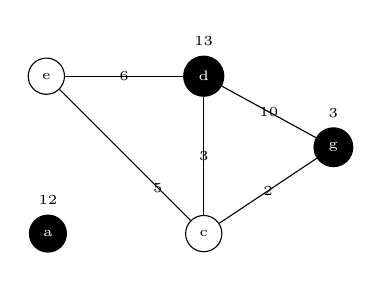
\begin{tikzpicture}[node distance=1.5 cm,
        every node/.style={minimum width=0, minimum height=0}]]
    % Nodes
    \node[terminal, label={12}] (a) at (0,0){a};

    \node[steiner] (c) [right=of a] {c};
    \node[terminal, label={13}] (d) [above =of c] {d};
    \node[steiner] (e) [left=of d] {e};
    \node[terminal, label={3}] (g) [above right=0.75 and 1.3 of c] {g};
    % Edges

    \draw (c) edge node{3} (d);
    \draw (c) edge node{2} (g);
    \draw (c) edge node[near start]{5} (e);
    \draw (d) edge node{6} (e);
    \draw (d) edge node{10} (g);
  \end{tikzpicture}};
\node[minimum width=5cm,
      minimum height=2.5cm] (5) at (0, -8) {
  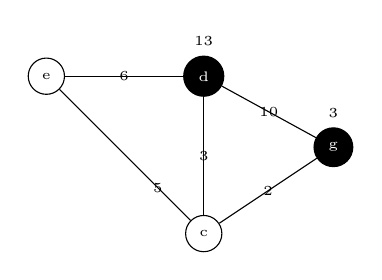
\begin{tikzpicture}[node distance=1.5 cm,
        every node/.style={minimum width=0, minimum height=0}]]
    % Nodes
    \node[terminal, draw=none, fill=none] (a) at (0,0){\phantom{a}};
    \node[steiner] (c) [right =of a] {c};
    \node[terminal, label={13}] (d) [above =of c] {d};
    \node[steiner] (e) [left=of d] {e};
    \node[terminal, label={3}] (g) [above right=0.75 and 1.3 of c] {g};
    % Edges

    \draw (c) edge node{3} (d);
    \draw (c) edge node{2} (g);
    \draw (c) edge node[near start]{5} (e);
    \draw (d) edge node{6} (e);
    \draw (d) edge node{10} (g);
  \end{tikzpicture}};
\node[minimum width=5cm,
      minimum height=2.5cm] (6) at (9, -8) {
        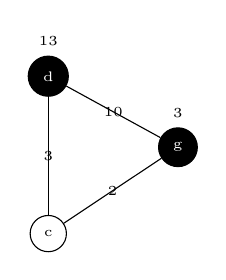
\begin{tikzpicture}[node distance=1.5 cm,
          every node/.style={minimum width=0, minimum height=0}]]
    % Nodes

    \node[steiner] (c) at (0,0) {c};
    \node[terminal, label={13}] (d) [above =of c] {d};
    \node[terminal, label={3}] (g) [above right=0.75 and 1.3 of c] {g};
    % Edges

    \draw (c) edge node{3} (d);
    \draw (c) edge node{2} (g);
    \draw (d) edge node{10} (g);
  \end{tikzpicture}
};
\node[minimum width=5cm,
minimum height=2.5cm] (7) at (0, -12) {
  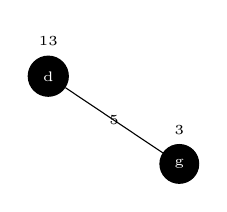
\begin{tikzpicture}[node distance=1.5 cm,
    every node/.style={minimum width=0, minimum height=0}]
    % Nodes
    \node[terminal, label={13}] (d) {d};
    \node[terminal, label={3}] (g) [below right=0.75 and 1.3 of d] {g};
    % Edges

    \draw (d) edge node{5} (g);
  \end{tikzpicture}};
\node[minimum width=5cm,
      minimum height=2.5cm] (8) at (9, -12) {
  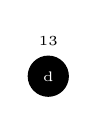
\begin{tikzpicture}[node distance=1.5 cm,
        every node/.style={minimum width=0, minimum height=0}]
    % Nodes
    \node[terminal, label={13}] (d) {d};
  \end{tikzpicture}};

% \draw [->,decorate, thick,
% decoration={snake,amplitude=.4mm,segment length=2mm,post length=1mm}]
% (1)
% edge node [above=1mm,midway,text width=3cm, sloped, align=center] {hej}
% (2);

\draw (1) edge[snake it] node[snake node] {1: $NTD_1$} (2);
\draw (2) edge[snake it] node[snake node] {2: $TD_1$} (3);
\draw (3) edge[snake it] node[snake node] {3: $MA$} (4);
\draw (4) edge[snake it] node[snake node] {4: $UV$} (5);
\draw (5) edge[snake it] node[snake node] {5: $NTD_2$} (6);
\draw (6) edge[snake it] node[snake node] {6: $NTD_2$} (7);
\draw (7) edge[snake it] node[snake node] {7: $TD_2 + UV$} (8);
\end{tikzpicture}
\caption{Graph reduction on the \gls{pcstp} instance in Figure \ref{fig:pcstp:01}. In the final graph,
 the node $d$ represents nodes $\{a,b,d\}$.}
\label{fig:pre:ex}
\end{figure}

This example shows how successive application of preprocessing routines can be at
reducing the size of an input graph. These routines have a cascading effect as one
graph reduction makes another one legal. In Figure (\ref{fig:pre:ex}) this comes to
pass when the third reduction -- the \textit{Minimum Adjacency} test -- contracts
the edge between nodes $b$ and $d$, causing the degree of nodes $c$ and $e$ to
 drop to 2, which allows for the fifth and sixth reductions.
\end{example}

It is an open question which selection of graph reduction tests are
 most efficient, and likewise with the ordering of graph reductions.
%%% Local Variables:
%%% TeX-master: "report"
%%% reftex-default-bibliography: ("lit.bib")
%%% End:


\clearpage
\clearpage
\section{Approximation Algorithms}\label{sec:solving:approx}

\subsection{The Goemans-Williamson Algorithm}\label{sec:solving:approx:gw}
\citet*{goemans1995general} presented a primal-dual 2-approximation algorithm for the rooted variant of the
\gls{pcstp}, based on an algorithm for solving the general \textit{constrained forest problem}.

\todo[inline]{Quick summary of usage. It is popular.}

\paragraph{Definitions}
\citeauthor{goemans1995general} stated the \gls{ilp} (GW-ILP) in Formulation \ref{form:approx:gw} for the rooted \gls{pcstp}.

 \begin{formulation}[h!]
   \begin{subequations}
     \begin{alignat}{3} 
       &\underset{x, z}{\text{minimize}}
       & & \sum_{e \in E} c_e x_e + \sum_{X \subset V; r \not\in X} z_X \left( \sum_{v \in X} p_v \right) & \\
       & \text{subject to}\quad
       & & x(\delta(S)) + \sum_{X \supseteq S}z_X \geq 1 \qquad&& \forall S \subset V; r \not\in S \label{form:approx:gw:cut}\\
       &&& \sum_{S \subset V; r \not\in S} z_X \leq 1 && \label{form:approx:gw:cz}\\
       &&& x_e \in \BB  && \forall e \in E \\
       &&& z_X \in \BB  && \forall S \subset V; r \not\in S
     \end{alignat}\label{form:approx:gw}
   \end{subequations}
   \caption{(GW-IP) formulation of the \gls{pcstp}.}
 \end{formulation}

 GW-IP has two decision vectors. The decision vector $x$ denotes which edges are contained in the solution,
 and the decision vector $z$, we have that $z_X$ is
 $1$ when iff. all $v \in X$ are not part of a feasible solution. Clearly, any optimal solution will have $z_X = 1$ for just a single
 $X \subset V$. However, it is still enforced by constraint (\ref{form:approx:gw:cz}).

 Constraint (\ref{form:approx:gw:cut})
 ensures that the solution is connected subgraph by requiring that for each subset $S$, the cut defined by $S$ must either be
 bridged by an edge in a feasible solution or $S$ must be counted as not included.

 \begin{formulation}[h!]
   \begin{subequations}
     \begin{alignat}{3} 
       &\underset{x, z}{\text{maximize}}
       & & \sum_{S \subset V; r \not\in S} y_S & \\
       & \text{subject to}\quad
       & & \sum_{S: e \in \delta(S)} y_S \leq c_e \qquad&& \forall e \in E \label{form:gw:pe}\\
       &&& \sum_{S \subseteq X} y_S \leq \sum_{v \in X} p_v  && \forall X \subset V; r \not\in X \label{form:gw:pv} \\
       &&& y_S \geq 0  && \forall S \subset V; r \not\in S
     \end{alignat}\label{form:approx:gw:dual}
   \end{subequations}
   \caption{(GW-D): Dual of the LP relaxation of (GW-ILP) from Formulation \ref{form:approx:gw}.}
 \end{formulation}
 
 The dual to the LP relaxation of GW-IP is the linear program in \ref{form:approx:gw:dual}. We make note of the
 \textit{packing} constraints (\ref{form:gw:pe}) and (\ref{form:gw:pv}), and note that by \textit{complementary slackness}
 of the primal LP, we have for optimal primal solutions to the LP, $(x^*, z^*)$,
 $$x^*_e > 0 \Rightarrow \sum_{S: e \in \delta(S)} y_S = c_e$$
 and
 $$z^*_X > 0 \Rightarrow \sum_{S \subseteq X} y_S = \sum_{v \in X} p_v\mathnormal{.}$$
 

 
 \paragraph{The Algorithm} The GW Algorithm consists of a growing phase and a pruning phase. The growing phase
 builds a feasible solution $T$ by maintaining a set of active and inactive \textit{components} which
 initially are singleton sets which are active if they do not contain the root vertex. The dual objective value is then
  increased by simultaneously increasing
  the dual variable values for all active components until one of the following happen:
 \begin{enumerate}[label=\alph*)]
 \item A packing constraint (\ref{form:gw:pe}) becomes binding for some edge $e = (i,j) \in E$. Then $e$ is added
   to $T$, and the components connected by $e$ are merged into a new component with combined cost.
   The new component is considered active iff the root vertex is not contained in it.
 \item A packing constraint (\ref{form:gw:pv}) becomes binding for some subset $X  \subset V$ (i.e. component). Then $X$ is deactivated
    and all vertices it contains are marked with the label $X$.
 \end{enumerate}
 This continues until there are no active components left; at which point $T$ is a feasible solution to the IP (GW-IP).

 
 \begin{algorithm}[h!]
   \begin{algorithmic}[1]
     \Input{Graph $G = (V, E, c, p)$ and root vertex $r \in V$.}
     \Output{Tree $T' \subseteq E$, and the set of vertices not spanned by $T'$, $X$.}
     \Procedure{GW Algorithm}{}
     \State $T \gets \emptyset$ \label{gw:init-start}
     \State $\mathcal{C} \gets \{\{v\} : v \in V\}$
     \For {$v \in V$}
       \State $d(v) \gets 0$
       \State $w(\{v\}) \gets 0$
       \State Unmark $v$.
       \If {$v = r$}
         \State $\lambda(\{r\}) \gets 0$
       \Else
         \State $\lambda(\{v\}) \gets 1$
       \EndIf
     \EndFor \label{gw:init-end}
     \While{$\{ C \in \mathcal{C} \mid \lambda(C) = 1\} \neq \emptyset$}
     \State $\epsilon_1 \gets \min_{i,j} \frac{c_{ij} - d(i) - d(j)}{\lambda (C_i) + \lambda(C_j)},
     \qquad i \in C_i, j \in C_j, C_i \neq C_j$ \label{gw:select-start}
     \State $\epsilon_2 \gets \min_{w} \sum_{v \in C_w} p_v - w(C_w), \qquad C_w \in \mathcal{C}$
     \State $\epsilon \gets \min(\epsilon_1, \epsilon_2)$ 
     \State $w(C) \gets w(C) + \lambda(C) \epsilon$ for all $C \in \mathcal{C}$ \label{gw:add-component}
     \State $d(v) \gets d(v) + \lambda(C) \epsilon$ for all $v \in C \in \mathcal{C}$ \label{gw:add-vertex}
     \If{$\epsilon = \epsilon_1$}
     \State Add $(i,j)$ to $T$: $T \gets T \cup \{(i,j)\}$
     \State Merge $C_i$ and $C_j$ to $C_{ij}$,
     $\mathcal{C} \gets \mathcal{C} \cup \{C_{ij}\} \setminus \{C_i, C_j\}$
     \State If $r \in C_{ij}$ then $\lambda(C_{ij}) \gets 0$ else $\lambda(C_{ij}) \gets 1$
     \State $w(C_{ij}) \gets w(C_i) + w(C_j)$
     \Else
     \State Deactivate $C_w$, $\lambda(C_w) \gets 0$
     \State Mark all $v \in C_w$ with the label $C_w$
     \EndIf
     \EndWhile
     \State $T' \gets \Call{Prune}{T, Labels}$ 
   \EndProcedure
 \end{algorithmic}
 \caption{The GW Algorithm}\label{approx:gw:alg}
 \end{algorithm}

 The growing phase of the GW Algorithm is shown in Algorithm \ref{approx:gw:alg}. Lines \ref{gw:init-start}-\ref{gw:init-end}
 initialise the set of components as described above -- only the component containing the root vertex is set as inactive.
 The lines \ref{gw:select-start}-\ref{gw:add-vertex} then determine the amount, $\epsilon$, which is
 the value that dual decision variables
 can be increased by for all active components
 until a packing constraint becomes binding. Since this behaviour is not directly clear for the definition of the algorithm itself,
  we attempt to give some intuition in the following.

 At the beginning of each iteration we have,
 $$d(v) = \sum_{S: v \in S} y_S, \forall v \in V \mathnormal{.}$$
 This follows directly from line \ref{gw:add-vertex}. Suppose that the corresponding
 packing constraint for the edge $e = (i,j)$ is
  the tightest ``active'' constraint. Notice that we can reformulate the left side of the constraint (\ref{form:gw:pe}) as follows,
 $$\sum_{S: (i,j) \in \delta(S)} y_S = \sum_{S : i \in S} y_S + \sum_{S : j \in S} y_S - \sum_{S : i,j \in S} y_S\mathnormal{.}$$
 Since we are only considering edges which connect components, we clearly must have $\sum_{S : i,j \in S} y_S = 0$
 and thus,
 $$\sum_{S: (i,j) \in \delta(S)} y_S = d(i) + d(j)\mathnormal{.}$$
 Suppose, w.l.o.g., that both $i$ and $j$ belong to active components.
 When the iteration is over, we will have increased $d(i)$ and $d(j)$ by $\epsilon = \frac{c_{ij} - d(i) - d(j)}{2}$.
 Then clearly the packing constraint for $e = (i,j)$ is then binding as demostrated below,
 $$\sum_{S: (i,j) \in \delta(S)} y_S = d(i) + \left( \frac{c_{ij} - d(i) - d(j)}{2} \right) + d(j) +
 \left( \frac{c_{ij} - d(i) - d(j)}{2} \right)   = c_{ij}\mathnormal{.}$$
 The case where a packing constraint (\ref{form:gw:pv}) is the tightest is similar, and follows directly from the loop
 invariant
 $$w(C) = \sum_{S \subset C} y_S, \forall C \in \mathcal{C}\mathnormal{.}$$

 The pruning phase of the algorithm is described by \citet{goemans1995general}
 as a procedure which removes as many
 edges from $T$ while upholding that:
 \begin{enumerate}
 \item any unlabeled vertex is connected to the root vertex, $r$, and
 \item if a vertex with label $C$ is connected to $r$ then any vertex with
   label $C' \supset C$ must also be connected to $r$.
 \end{enumerate}
 This pruning procedure was improved upon by the ``strong pruning'' procedure introduced by \citet{Johnson:2000:PCS:338219.338637},
  which we will detail in Section \ref{sec:approx:strongpruning}.
 \paragraph{Analysis}
 The GW Algorithm is proven to produce a result which is less than twice as bad as an optimal solution to (GW-IP), $Z^*_{\text{GW-IP}}$, and thus
 is a 2-approximation algorithm. This follows from the following inequality,
 $$\sum_{e \in T'}c_e + \sum_{v \in X} p_v \overset{\text{(I)}}{=}   \sum_{e \in T'} \sum_{S: e \in \delta(S)} y_S  + \sum_{j} \sum_{S \subseteq C_j} y_S
 \overset{\text{(II)}}{\leq} (2 - \frac{1}{n-1}) \sum_{S \subset V} y_S \overset{\text{(III)}}{\leq} (2 - \frac{1}{n-1}) Z^*_{\text{GW-IP}}\mathnormal{.}$$
 The reader is encouraged to read \citet{goemans1997primal} for the full proof, but it roughly goes as follows:
 \begin{itemize}
 \item (I) holds from primal complimentary slackness. An edge is only added to $T$ if its corresponding packing constraint is binding.
   Additionally, for a vertex to not be spanned by $T$, it must have been deactivated at some point during the
    algorithm (and thus the corresponding packing constraint must have
    been binding).
  \item (II) holds from an induction proof on main loop of the procedure, and
  \item (III) holds from the feasibility of the $y$ vector which is implicitly procduced by the procedure and then weak duality.
 \end{itemize}
 Furthermore, the GW Algorithm is proven to run in $O(n^2 \log n)$.
 \subsection{Modifications to the GW Algorithm}\label{sec:approx:strongpruning}
 \citet{Johnson:2000:PCS:338219.338637} investigated three main modifications to the GW Algorithm:
 \begin{enumerate}
 \item an improved pruning procedure called Strong Pruning,
 \item how the algorithm performs on the unrooted \gls{pcstp}, and
 \item how pertubation of the prize vector affects the algorithm.
 \end{enumerate}
 Furthermore, as a part of these investigations, they produced an implementation of the GW Algorithm.
 In this section we will detail the Strong Pruning procedure, and touch upon the results from the two other
  investigations.
 \paragraph{Strong Pruning} The Strong Pruning procedure
 (as shown in Algorithm \ref{alg:approx:gwsp})
 is a simple recursive procedure which walks the tree in post-order while calculating the net-worths
 of all subtrees. If --- along the way --- a subtree is encountered which is connected by an
  edge which has higher cost than the net-worth of the subtree, then the subtree is discarded.
 \begin{algorithm}[h!]
   \begin{algorithmic}[1]
     \Input{Feasible solution to (GW-IP), $T$ rooted in vertex $r$ to $G = (V, E, c, p)$} 
     \Output{A tree $T' \subseteq E$.}
     \State $T' \gets T$
     \Procedure{StrongPrune}{r}
     \State $nw(r) \gets p_r$
     \For{$v \in \Call{Children}{r}$}
     \State \Call{StrongPrune}{v}
     \If{$nw(v) \leq c_{rv}$}
     \State $T' \gets T' \setminus \{(r,v)\}$
     \Else
     \State $nw(r) \gets nw(r) + nw(v) - c_{rv}$
     \EndIf
     \EndFor
   \EndProcedure
 \end{algorithmic}
 \caption{Strong pruning for the GW Algorithm.}\label{alg:approx:gwsp}
\end{algorithm}

The Strong Pruning procedure clearly runs in $O(n)$ time, which is an improvement on the $O(n^2)$
guarantee for the pruning procedure presented by \citet{goemans1995general}. Additionally,
Strong Pruning does not require any additional information about the candidate solution, $T$,
which is in contrast with the labels required by the GW Pruning procedure.

However, computational experiments performed by \citet{Johnson:2000:PCS:338219.338637}
do not report any significant speedup gained by replacing GW Pruning with
Strong Pruning in the GW Algorithm
as the algorithm is dominated by its $O(n^2 \log n)$ growing phase.

However, they do report
improvements in objective value. On 12 instances based on street maps,
the vanilla GW Algorithm produced objective values which are in the range of $2-9\%$
worse than those produced by the GW Algorithm modified with Strong Pruning. On randomly
generated instances, this is reported to be up to $20\%$.

Thus, modifying the GW Algorithm to perform Strong Pruning results in better solutions at
 no extra cost.
\paragraph{GW  Algorithm for the unrooted \gls{pcstp}}
The GW Algorithm is stated and its approximation ratio proved
for the rooted variant of the \gls{pcstp}. While these apply directly to unrooted variants
when run for all possible roots, this comes with
a worsened $O(n^3 \log n)$ runtime.

\citet{Johnson:2000:PCS:338219.338637} verify that if the growth phase of the GW Algorithm
is replaced with a procedure which does not treat the root vertex as special, both the
approximation ratio and asymptotic runtime proven for the rooted variant are still valid.

Computationally, however, they report a $1.5-2.0$ slowdown for a unrooted GW Algorithm. They also
report that running the rooted GW Algorithm repeatedly with randomly selected roots give slightly
better objective value (less than $1\%$ difference) than the unrooted variant, although at a starkly
higher cost.
\paragraph{Prize Pertubation} The third thing investigated by \citet{Johnson:2000:PCS:338219.338637} was
the effect of pertubing vertex prizes by some constant $\alpha$, that is setting
$$p_v \gets \alpha p_v$$
for all $v \in V$. This ``tricks'' the GW Algorithm into over/undervaluing the importance of gathering prizes,
 leading to altered behaviour.

 Experiments performed by \citeauthor{Johnson:2000:PCS:338219.338637} resulted in $\alpha \approx 0.85$ giving a $\sim2\%$
 lower objective values compared to $\alpha = 1$ for the GW Algorithm with Strong Pruning on random instances.
  This kind of prize pertubation is explored further by \citet{canuto2001local} -- see Section \ref{sec:canuto-search}.


%%% Local Variables:
%%% TeX-master: "report"
%%% reftex-default-bibliography: ("lit.bib")
%%% End:


\section{Heuristics}\label{sec:solving:heuristics}

\subsection{Local Search with Pertubation and Relinking}\label{sec:canuto-search}

\cite{canuto2001local} presented a multi-phase heuristics which makes use of the GW Algorithm.
 Algorithm \ref{alg:heuristics:canuto} sketches the full procedure. 

 The heuristics can be seen as a multi start heuristics which uses the GW Algorithm
 to generate good intitial
 solutions (line \ref{alg:canuto:line:gw})
 which it progressively refines using using a hill climbing local search
 (line \ref{alg:canuto:line:hc}),
 and then a path relinking scheme against a previous good solution
 (line \ref{alg:canuto:line:relink}).
 Pertubation of the prize vector, $p$, is used to push the GW Algorithm to generate
 different solutions on multiple starts, and finally, a
 variable neighbourhood search is applied as a
 post processing step to refine the best candidate solution found.

 \begin{algorithm}[h!]
   \begin{algorithmic}[1]
     \Input{Graph $G = (V, E, c, p)$.}
     \Output{Tree $\tilde{T} \subseteq G$.}
     \Procedure{Canuto-LocalSearch}{}
     \State $E \gets \emptyset$, $\hat{p} \gets p$, $\hat{z}^* \gets \infty$
     \For{$i \in 1...\mathit{max\_iterations}$}
     \State $S \gets \Call{GW-Algorithm}{V,E, c, \hat{p}}$ \label{alg:canuto:line:gw}
     \If{$S$ hasn't been seen in previous iterations}
     \State $S' \gets \Call{Hill-Climbing}{S', G = (V, E, c, p)}$ \label{alg:canuto:line:hc}
     \State Add $S'$ to $E$ if it satisfies the necessary criteria \label{alg:canuto:line:elite}
     \State Pick random $Y \in E$
     \State $S' \gets \Call{Relink}{S', Y}$ \label{alg:canuto:line:relink}
     \If{$c(S') < \hat{z}^*$}
     \State $\hat{z}^* \gets c(S')$
     \State $S^* \gets S'$
     \EndIf
     \EndIf
     \State Pertubate $\hat{p}$
     \EndFor
     \State $S^* \gets \Call{VNS}{S^*, G = (V, E, c, p)}$\label{alg:canuto:line:vns}
     \State \Return $\Call{MST}{G[S^*]}$
     \EndProcedure
 \end{algorithmic}
 \caption{The heuristics defined by \cite{canuto2001local}.}\label{alg:heuristics:canuto}
 \end{algorithm}

 In this section we will
 describe further the characteristics of the local search, the
 path relinking, and the postprocessing used in the algorithm.
\paragraph{Local Search with Pertubations}
\cite{canuto2001local} define their search space as the space of minimum spanning
trees on all graphs induced by a subset of vertices
 $S \subset V$. If $G[S]$ is the subgraph induced by the vertex subset $S \subseteq V$, then
 this search space can formally be defined as
$$\mathcal{S_G} = \{MST(G[S]) : S \subseteq V \}\mathnormal{.}$$
A neighbour to a given MST is then any MST of a subgraph induced by a subset which differs from $S$
 by exactly one vertex, that is,
$$\mathcal{N}(S) = \Big\{MST(G[S']) : S' \subseteq V \Bigm| |S' \triangle S| = 1 \Big\}\mathnormal{.}$$ 
Clearly this neighbourhood structure means that all feasible solutions are reachable
given any initial subset as starting point. Additionally, they define the
$k$'th order neighbourhood as,
$$\mathcal{N}^k(S) = \Big\{MST(G[S']) : S' \subseteq V \Bigm| |S' \triangle S| = k \Big\}\mathnormal{.}$$ 

To reduce clutter we will denote the cost
of a given subset, $S \subseteq V$, of vertices as the cost
of the MST of the graph induced by $S$, that is
$$c(S) = c(MST(G[S]))\mathnormal{.}$$

The search algorithm itself is just a plain hill-climbing algorithm which repeatedly
 moves to the first
 found neighbouring solution with lower cost until it arrives at a local minima.

 To overcome the problem of running into the same local minima repeatedly,
 \cite{canuto2001local} employ two pertubation schemes which are alternately applied
 on even and odds iterations:
 \begin{enumerate}
 \item A fixed percentage of vertices which have appear both in the initial solution generated
   by the GW Algorithm \textit{and}  in the solution subsequently generated by
    the hill climbing procedure have their prizes
    set to zero.
  \item A pertubation factor, $\alpha$, is randomly picked within a fixed interval $[1 -a, 1+a]$
    and prizes are set to $p_v \gets \alpha p_v$ for all $v \in V$.
 \end{enumerate}

\paragraph{Path Relinking}
For every iteration of the main loop, the relinking procedure in Algorithm \ref{heuristics:canuto:relink}
is applied to a solution generated by the hill climbing procedure and 
a random \textit{elite} solution which is picked from the
persistant pool of elite solutions, $E$.

The relinking procedure basically transforms $S$ into $Y$ one vertex at a time in a greedy fashion.
The solution along the way which has the best objective value is then returned.
 \begin{algorithm}[h!]
   \begin{algorithmic}[1]
     \Procedure{Apply}{S, v}
     \If{$v \in S$}
     \State \Return $S \setminus \{v\}$
     \Else
     \State \Return $S \cup \{v\}$
     \EndIf
     \EndProcedure
     \Procedure{Relink}{S, Y}
     \State $D \gets S \triangle Y$
     \State $S' \gets S$
     \State $\tilde{S} \gets S$
     \While{$S' \neq Y$}
     \State $v^* \gets \argmin_{v \in D} c(\Call{Apply}{S,v})$
     \State $S' \gets \Call{Apply}{S', v^*}$
     \State if $c(S') < c(\tilde{S})$ then set $\tilde{S} \gets S'$
     \State $D \gets D \setminus \{v\}$
     \EndWhile
     \State \Return $\tilde{S}$
     \EndProcedure
 \end{algorithmic}
 \caption{The relinking scheme used by \cite{canuto2001local}.}\label{heuristics:canuto:relink}
 \end{algorithm}

 Entry into $E$ for a subset $S$ is dermined by two criteria:
 either we must
 $$c(\tilde{S}) < \min_{S \in E} c(S)\mathnormal{,}$$
 or we must have both
 $$c(\tilde{S}) < \max_{S \in E} c(S)$$
  and that the Hamming distances between the characteristic vectors of $\tilde{S}$
   and \textit{all} solutions in $E$ are greater than $\rho |V|$ for some $\rho \leq 1$. 

\paragraph{Postprocessing}
Variable neighbourhood search (VNS) (See \cite{hansen2010variable}) is applied
to best candidate solution as a post-processing step. In principle, the VNS
procedure (shown in Algorithm \ref{alg:heuristics:canuto:vns}) is a hill climbing
search within a union of the first $k_{max}$ order neighbourhoods with an early stopping
 criteria.
\begin{algorithm}[h!]
   \begin{algorithmic}[1]
     \Procedure{VNS}{S}
     \For{$i \in 1...\mathit{max\_iterations}$}
     \State $k \gets 1$
     \While{$k  \leq k_{max}$}
     \State Pick random $S' \in \mathcal{N}^k(S)$
     \State $\tilde{S} \gets \Call{Hill-Climbing}{S'}$
     \If{$c(\tilde{S}) < c(S)$}
     \State $k \gets 1$
     \State $S \gets \tilde{S}$
     \Else
     \State $k \gets k + 1$
     \EndIf
     \EndWhile
     \EndFor
     \State \Return $S$
     \EndProcedure
 \end{algorithmic}
 \caption{The Variable Neighbourhood Search
   used by \cite{canuto2001local}.}\label{alg:heuristics:canuto:vns}
 \end{algorithm}

 As a postprocessing step, this procedure is only applied to the single best solution generated
  by all the the previous steps.
\paragraph{Evaluation}
Based on the implementation of the GW Algorithm by \cite{Johnson:2000:PCS:338219.338637},
\cite{canuto2001local} performed experiments, detailing the objective function value
and running time of
\begin{itemize}
\item The GW Algorithm,
\item The multi-start local search procedure with pertubations
\item The above combined with path relinking, and
\item The full heuristics.
\end{itemize}

All three ``parts'' of the heuristics are shown to help improve upon the
objective value generated by the previous parts.
But in particular, \citeauthor{canuto2001local} report that adding the
path relinking scheme results in a stark increase
 in number of instances solved to optimality.


%%% Local Variables:
%%% TeX-master: "report"
%%% reftex-default-bibliography: ("lit.bib")
%%% End:


\section{Lower Bounding Procedures}
\label{sec:solving:lower}

\subsection{Generalised Subtour Elimination Constraints}
\label{sec:lower:gsec}
\cite{lucena2004strong} introduced a method for producing lower bounds for the PCSTP based on solving
the LP relaxations of the PCSTP using a constraint separation procedure.

Their main contributions
are the stating of a \textit{generalised subtour elimination constraint} ILP (see Formulation \ref{form:lower:gsec}) formulation
for the PCSTP, the separation procedure for solving the LP-relaxation, and strengthening of the formulation by considering
single vertex solution seperately.

Define the function
$$E(S) = \{(i,j) \in E \mid i \in S \wedge j \in S\}$$
then Formulation (\ref{form:lower:gsec}) is a ILP formulation of the PCSTP. Constraints (\ref{form:lower:gsec:gsec}) are
referred to as generalised subtour elimination constraints, and together with constraint (\ref{form:lower:gsec:sum})
ensure that the solution defined by $(x, y)$ is a tree which spans the vertices $y_v = 1$.

 \begin{formulation}[h!]
   \begin{subequations}
     \begin{alignat}{3} 
       &\underset{x,y}{\text{minimize}}
       & & \sum_{e \in E} c_e x_e +  \sum_{v \in V} p_v (1 - y_v)  & \\
       & \text{subject to}\quad
       & & x(E) \leq y(V) - 1 &&  \label{form:lower:gsec:sum}\\
       &&& x(E(S)) \leq y(S \setminus \{s\}) && \forall s \in S, S \subseteq V \label{form:lower:gsec:gsec}\\
       \intertext{ILP:}
       &&& x_e \in \BB  && \forall e \in E \\
       &&& y_v \in \BB  && \forall v \in V \\
       \intertext{LP:}
       &&& 0 \leq x_e \leq 1  && \forall e \in E \\
       &&& 0 \leq y_v \leq 1  && \forall v \in V \\
       \intertext{To exclude single vertex solutions:}
       &&& \sum_{i \in \delta(v)} x_{vi} \geq
       \begin{cases}
         y_v & p_v > 0 \\
         2y_v & p_v = 0
       \end{cases} \qquad && \forall v \in V \label{form:lower:gsec:single}
     \end{alignat}\label{form:lower:gsec}
   \end{subequations}
   \caption{(GSEC-IP) GSEC formulation of the PCSTP.}
 \end{formulation}

 Expanding the formulation with constraint (\ref{form:lower:gsec:single}), excludes single vertex solutions.
 \cite{lucena2004strong} found that adding these constraints and
 considering single vertex solutions in a separate routine results faster runtimes.

 \paragraph{Separation of GSECs} Each subset $S \in V$ produces $|S|$ GSECs. To reduce the size of the LP relaxation,
 \cite{lucena2004strong} suggest relaxing these constraints and readding them in a separation procedure.
 This separation procedure can be stated a max-flow problem as follows:

 Let $(\bar{x}, \bar{y})$ be a solution to the relaxed LP. Consider the support graph induced by vertices and edges with nonzero decision veriables,
  and vertex $l$ with decision variable $\bar y_l > 0$
  then iff
  $$\max_{S_l \subseteq V} \left\{ \bar x (E(S_l)) - (\bar y (V) - \bar y_l) \right\} > 0$$
  there is a violated GSEC for a subset containing $l$, and constraint corresponding to $S_l^{max}$ is the most violated constraint.

  We can model finding this subset for a given $l$ as follows. Let $\bar{N} = (\bar{V}, \bar{A})$ be a flow-network
  for the support graph, with vertices
  $$\bar V = \{s, t\} \cup \{v \in V \mid \bar y_v > 0 \}$$
  and arcs
  $$\bar A = \{(i, j) \in E \mid \bar x_{ij} > 0 \} \cup \{(j, i) \in E \mid \bar x_{ij} > 0\} \cup \{(s, v) \mid v \in \bar V\} \cup \{(v, t) \mid v \in \bar V\}\mathnormal{.}$$
  Additionally we have capacities original edges,
  $$\xi_{ij} = \xi_{ji} = \frac{\bar x_{ij}}{2} \qquad \forall (i,j) \in \bar A$$
  and if we let $\delta (v)$ be all vertices adjacent to $v$ in the support graph then node capacities are
  $$\xi_v = \sum_{u \in \delta(v)} \xi_{vu}\mathnormal{,}$$
  and finally
  for arcs from and to the source and the sink, we have
  $$\xi_{sv} =
  \begin{cases}
    \infty & v = l \\
    \max(\xi_v - \bar y_v, 0) & \text{otherwise}
  \end{cases}$$
  and
  $$\xi_{vt} = \max(\bar y - \xi_v, 0)\mathnormal{.}$$
  Then the minimum $(S,T)$ cut on the flow network will minimise
  $$\sum_{v \in S} \max \left\{\bar y_v - \xi_v, 0\right\} + \sum_{i \in S, j \in T} \bar x_{ij} + \sum_{v \in T} \max\left\{\bar \xi_v - y_v, 0\right\}\mathnormal{.}$$
  In effect, we have added the negative part of $\bar y_v - \xi_v$ to all subsets, $S$, which don't contain $v$. This makes the above equivalent to
   minimising
  $$\sum_{v \in S} (\bar y_v - \xi_v) + \sum_{i \in S, j \in T} \bar x_{ij} = \sum_{v \in S} \bar y - \sum_{e \in E(S)} \bar x$$
  which in turn maximises
  $$\sum_{e \in E(S)} \bar x - \sum_{v \in S} \bar y + \bar y_l \mathnormal{.}$$
  Hence any set of vertices $S' = S \setminus \{s\}$ where $S$ induces a minimal $S,T$ cut in the flow network will correspond to
  a most violated GSEC for the solution $(\bar x, \bar y)$ to the relaxed LP.

  Finding violated GSECs then reduces to solving $|V|$ maximum flow problems, which can be done in polynomial time. However, there is guarantee that
  that the $|V|$ will result in different violated constraints. To avoid this, \cite{lucena2004strong} suggest that whenever a max-flow problem has been
  solved for some $l = v \in V$, then we can set $\xi_{vt} = \infty$ to avoid $v$ being on the source-side of any subsequent min-cuts.
  \todo[inline]{Wolsey (I think) suggests deleting edges/vertices from the support graph, maybe mention that}
  
\section{Exact Algorithms}\label{sec:solving:exact}

\subsection{DHEA Solver}
\label{sec:exact:dhea}

\subsection{SCIP-Jack Solver}
\label{sec:exact:scipj}

%%% Local Variables:
%%% TeX-master: "report"
%%% reftex-default-bibliography: ("lit.bib")
%%% End:

\chapter{Research in Related Problems}
\label{chap:related}
*some motivation*
\todo[inline]{Do examples for this section. Show the problems.}

\section{The Steiner Tree Problem}
\todo[inline]{This section should be a section which highlights the research history of the STP
 which has been ``replicated'' in the PCSTP}
\section{The Prize-Collecting Travelling Salesman Problem and Variants}
\todo{Think about whether there should be a super-section about all the variants}
First introduced by \citet*{balas1989prize}, the Prize-Collecting Travelling Salesman Problem
(PCTSP) is a problem closely related to the
PCSTP.

The problem is formulated by \citeauthor{balas1989prize} as follows. Let
$G = (V, A, c, p)$ be a directed
graph with arc costs $c: A \to \RR_+$ and vertex prizes (or penalties) $p: V \to \RR_+$
then find a cycle $C = (V_C, A_C)$ with $V_C \subseteq V$ and $A_C \subseteq A$ which
minimises the function
$$\sum_{ij \in V_C} c_{ij} + \sum_{v \in V \setminus V_C} p_v$$
such that
$$\sum_{v_i \in V_C} p_i \geq B$$
for some $B \in \RR_+$.

If we recollect the definition of the PCSTP and its variants (Section \ref{sec:pcstp}) then
we immediately see some similarities. The PCTSP involves optimising the
\textit{Goemans-Williamson Minimization Problem} for the circuit $C$, however with the extra
constraint of collecting at least $B$ prize on the tour. This extra constraint draws comparisons
to the \textit{Quota Problem}.

As the PCTSP is a natural member of the family of Vehicle Routing Problems, it is also sometimes
stated with a \textit{depot} vertex \citep{feillet2005traveling} -- that is a vertex which
must be part of the solution cycle, $C$. This corresponds to the \textit{Rooted}
Prize-Collecting Steiner Tree Problem.

\paragraph{The Orienteering Problem}
The Orienteering Problem (OP) is very much the circuit version of the \textit{Budget Problem}.
Given a graph $G  = (V, E, c, p)$, the OP inolves finding a circuit, $C = (V_C, E_C)$,
which maximises
$$\sum_{v \in V_C}  p_v \quad \text{s.t.} \quad \sum_{ij \in E_C} c_{ij} \leq B$$
for some $B \in \RR_+$.
\todo{Add something short on the history of the OP}
\paragraph{The Profitable Tour Problem}
A maybe more familiar problem in the realm of prize collecting tour problems, is the
so-called Profitable Tour Problem (PTP). This variant -- which earlier shared name with
the PCTSP -- involves dropping the quota constraint from the PCTSP, making it a true
 ``cousin'' of the PCSTP.

 While similar in formulation to the PCSTP, according to a fairly recent survey by
 \citet{archetti2014chapter}, the PTP has received very little attention -- 
 especially when compared to the PCSTP.
 In fact, to the best of our knowledge, no exact solution to the PTP
 has been proposed outside the lower bounding procedure proposed by \citet{dell1995prize},
  which is a big step in defining an exact algorithm.
 
 However, there has been some research into approximation algorithms for the PTP.
 In fact, an interesting symptom of exactly how related these two families of
 prize collecting problems are
is how the GW Algorithm (see Section \ref{sec:solving:approx:gw})
can be used used to generate a 2-approximation algorithm for the PTP
on graphs satisfying the triangle inequality in the same way as
polynomial time MST algorithms can be used to generate 2-approximation algorithms
for the TSP \citep{goemans1995general}.



 \section{The Median Facility Problems}
 A type of problems which are closesly related to the ``prize-collecting'' problems such as the PCSTP, are the so-called
 ``median'' problems. These problems involve finding optimal location of a ``facility'' with regards to the sum
 of distances from all vertices to the facility.

 For example, first introduced in \citeyear{hakimi1964optimum} by \citet{hakimi1964optimum} is a problem known as
 the \textit{$p$-Median Problem}. Given a graph $G = (V, E, c)$, this involves selecting a subset $S \subseteq V$ with
 cardinality $p$ such that $S$ minimises the sum of minimum distances from vertices in $V$ to vertices in $S$.
 
 \citet{current1987median} adds structure to the selection of vertices by introducing the \textit{Median Shortest Path Problem (MSPP)}.
 Here, given a graph $G = (V,E,c,d,p)$ -- where $c$ and $d$ are edge weight functions --
 and source and sink vertices $s$ and $t$, one must find a facility
  -- now a simple path $P$ --  in $G$
 from $s$ to $t$ in s.t. the function
 $$\sum_{i,j \in E(P)} c_{ij} + \sum_{i \in V} p_i D_{i, P}$$
 where $p_i$ is the weight of vertex $v_i$ and
 $D_{i, P}$ is the shortest path from vertex $v_i$ to any vertex in $P$ with regards to
 weights $d$.
 We commonly denote the first sum as the cost of the facility/subgraph and the second sum as the assignment cost.

 Intuitively, the MSPP involves weighing a trade off between the cost of the facility
 in $c$ and the assignment costs. 
 This is analogous to the trade off between the cost of a subgraph and the cost of missed prize in the
 family of prize-collecting problems. In the median problems, the fixed prize of a vertex is
 replaced by the variable ``prize'' represented by the shortest path to the facility sometimes weighted
 by a vertex prize.
 \subsection{The Median Ciruit/Tour Problem}
 The problem of finding a circuit shaped facility in a graph has also been studied.
 \citet{labbe1999themedian} introduced the ``Median Cycle Problem'' which involves
 minimising the cost of a cycle and assignment cost in a mixed graph (undirected for
 the facility and directed for assignment) given a root vertex. Alongside this problem
 -- which they denote (MCP1) -- they also introduced a budget version (MCP2) where the
 assignment cost minimisation is replaced with a constraint, and branch-and-cut algorithm
 were stated for them both.

 Additional research has been performed into both MCP varients
 in the form of new heuristics based on variable neighbourhood tabu search
 (similar to the methods used for the PCSTP by \citet{canuto2001local} --
 See Section \ref{sec:canuto-search}) by \citet{perez2003variable}, and both
 greedy and evolutionary heuristics were proposed by \citet{renaud2004efficient}.
 
 \citet{current1994median} introduced a similar problem named the ``Median Tour Problem''
 which is defined on a directed graph which has two edge cost functions and vertex prizes
 and involves optimising a bicriterion objective function
 (facility cost and prize-weighted assignment cost)
 when defining a cycle facility which spans a minimum number of vertices.

 The Profitable Tour Problem turns out to be a special case of certain variants of Median
 Tour Problems. Consider a variant defined as follows:

 Let $G = (V, E, c, d)$ be a undirected graph with two edge cost functions
 $c : E \to \RR$ and $d : E \to \RR$, then find a circuit $C = (V_C, E_C) \subseteq G$
 which minimises
 the function
 $$c(C) = \sum_{ij \in E_C} c_{ij} + \sum_{i \in V} \min_{j \in C} d_{ij} \mathnormal{.}$$
 Given this definition and an instance of the PTP on a graph $G = (V, E, c, p)$
 we can define an assignment cost function as
 $$d_{ij} =
 \begin{cases}
   0 & i = j \\
   p_i & i \neq j
 \end{cases}\mathnormal{.}
 $$
 Thus the assignment cost of a vertex is 0 if it is part of the facility and its prize
 if it is not.
 \subsection{The Median Subtree Problem}
*short history*

*problem definition*

*MIP Formulation*

*Maybe motivate a Median Steiner Problem*

%%% Local Variables:
%%% TeX-master: "report"
%%% reftex-default-bibliography: ("lit.bib")
%%% End:


\part{Exploration}

\chapter{The Median Tree Problem}
\label{chap:mediantree}

\section{Problem Defintion}

\section{Integer Programming Formulation}

\section{Implementation}

\section{Computational Experience}

\subsection{Instances}

\subsection{Results}


%%% Local Variables:
%%% TeX-master: "report"
%%% reftex-default-bibliography: ("lit.bib")
%%% End:

\makeatletter
\def\toclevel@chapter{-1}
\makeatother
\chapter{Conclusions}

\section{Future Work}

\textit{DiGraph transformation of \gls{mtp}.}
\textit{Produce real world datasets / datasets which represent different flavours of mtp}
\textit{Develop a strong heuristic for the MTP}
\textit{Reimplement the solver with system programming callbacks}

\section{Conclusion}


%%% Local Variables:
%%% TeX-master: "report"
%%% reftex-default-bibliography: ("lit.bib")
%%% End:


\phantomsection
\addcontentsline{toc}{part}{Bibliography}
\bibliographystyle{plainnat}
\bibliography{lit.bib}
\end{document}
